\documentclass[12pt]{report}
\usepackage{adjustbox}

\usepackage[T1]{fontenc}
\usepackage[utf8]{inputenc}
\usepackage{caption}
\usepackage{adjustbox}
\usepackage{graphicx}
\usepackage{amsmath,amssymb,amsfonts}
\usepackage{txfonts}
\usepackage{listings}
\usepackage{float}
\usepackage{color}
\usepackage{xcolor}
\usepackage{enumitem}
\usepackage{amsmath}
\usepackage{relsize}
\usepackage{tabularx}
\usepackage{microtype}

\setcounter{tocdepth}{1}
\setcounter{page}{5}
\graphicspath{{images/}}
\newcommand\setrow[1]{\gdef\rowmac{#1}#1\ignorespaces}
\renewcommand{\chaptername}{Rozdział}
\renewcommand{\contentsname}{Spis treści}
\renewcommand{\figurename}{Rysunek}
\renewcommand{\listfigurename}{Spis rysunków}
\renewcommand{\bibname}{Bibliografia}
\newtheorem{definition}{Definicja}
\newtheorem{example}{Przykład}[chapter]
\setlength{\textwidth}{14cm}
\setlength{\textheight}{20cm}
\hyphenation{thatshouldnot}
\captionsetup{justification=centering,margin=0cm}
\lstdefinelanguage{JavaScript}{
  keywords={typeof, new, true, false, catch, function, return, null, catch, switch, var, if, in, while, do, else, case, break},
  keywordstyle=\color{blue}\bfseries,
  ndkeywords={class, export, boolean, throw, implements, import, this},
  ndkeywordstyle=\color{darkgray}\bfseries,
  identifierstyle=\color{black},
  sensitive=false,
  comment=[l]{//},
  morecomment=[s]{/*}{*/},
  commentstyle=\color{purple}\ttfamily,
  stringstyle=\color{red}\ttfamily,
  morestring=[b]',
  morestring=[b]"
}
\lstset{
   language=JavaScript,
   backgroundcolor=\color{lightgray},
   extendedchars=true,
   basicstyle=\footnotesize\ttfamily,
   showstringspaces=false,
   showspaces=false,
   numbers=left,
   numberstyle=\footnotesize,
   numbersep=9pt,
   tabsize=2,
   breaklines=true,
   showtabs=false,
   captionpos=b
}
\lstdefinelanguage{XML}
{
  morestring=[b]",
  morestring=[s]{>}{<},
  morecomment=[s]{<?}{?>},
  stringstyle=\color{black},
  identifierstyle=\color{blue},
  keywordstyle=\color{cyan},
  morekeywords={xmlns,version,type}
}
\lstset{
  basicstyle=\ttfamily,
  columns=fullflexible,
  showstringspaces=false,
  commentstyle=\color{gray}\upshape
}
\colorlet{punct}{red!60!black}
\definecolor{background}{HTML}{EEEEEE}
\definecolor{lightgray}{rgb}{.9,.9,.9}
\definecolor{darkgray}{rgb}{.4,.4,.4}
\definecolor{purple}{rgb}{0.65, 0.12, 0.82}
\definecolor{delim}{RGB}{20,105,176}
\colorlet{numb}{magenta!60!black}
\lstdefinelanguage{json}{
    basicstyle=\normalfont\ttfamily,
    numbers=left,
    numberstyle=\scriptsize,
    stepnumber=1,
    numbersep=8pt,
    showstringspaces=false,
    breaklines=true,
    frame=lines,
    backgroundcolor=\color{background},
    literate=
     *{0}{{{\color{numb}0}}}{1}
      {1}{{{\color{numb}1}}}{1}
      {2}{{{\color{numb}2}}}{1}
      {3}{{{\color{numb}3}}}{1}
      {4}{{{\color{numb}4}}}{1}
      {5}{{{\color{numb}5}}}{1}
      {6}{{{\color{numb}6}}}{1}
      {7}{{{\color{numb}7}}}{1}
      {8}{{{\color{numb}8}}}{1}
      {9}{{{\color{numb}9}}}{1}
      {:}{{{\color{punct}{:}}}}{1}
      {,}{{{\color{punct}{,}}}}{1}
      {\{}{{{\color{delim}{\{}}}}{1}
      {\}}{{{\color{delim}{\}}}}}{1}
      {[}{{{\color{delim}{[}}}}{1}
      {]}{{{\color{delim}{]}}}}{1},
}

\begin{document}
\tableofcontents
\chapter{Wstęp}

  \section{Cel pracy}
    Celem pracy jest przedstawienie różnic, podobieństw oraz wspólnych konceptów między wybranymi frameworkami technologii Node.js.
    Od momentu jej ukazania się powstało wiele narzędzi ułatwiających oraz poprawiających jakość procesu deweloperskiego.
    Niektóre z nich skupiają się na usprawnianiu podobnych, pokrewnych lub identycznych przypadków użycia.
    Aby unkinąc nie trafnego wdrożenia wybranego narzędzia w opracowywany projekt, należy rozumieć kiedy wybrana metoda sprawdzi się najlepiej, a kiedy warto zastosować inne rozwiązanie.
    Nawet w przypdaku użycia tego samego języka programowania przeniesienie aplikacji pomiędzy frameworkami może być kosztownym oraz czasochłonnym zadaniem.
    Z tego powodu powstała potrzeba zakreślenia, które wyjście najlepiej sprawdza się dla określonego projektu lub jego części.
    W pracy zostały zawarte kryteria wyboru technologii, specyfikacje ocenianych parametrów, analiza frameworków oraz podsumowanie przeprowadzonych badań.

  \section{Przeznaczenie technologii Node.js}
    Node.js jest cross-platformowym, działającym niezależnie od środowiska językiem programowania, napisanym w językach c/c++ oraz javaScript, wydanym 27 marca 2009 roku, zaprojektowanym przez Ryana Dahla.
    Początkowym przeznaczeniem technologii było tworzenie serwerów i narzędzi sieciowych, działających po stronie serwera, lecz wraz z jej rozpowszechnieniem się możliwości te znacznie się poszerzyły oferując wytwarzanie między innymi aplikacji desktopowych (Electron), mobilnych (React Native, Cordova) lub rozwiązań embedded (Onoff).
    Przed jej powstaniem powstaniem kod w języku javaScript był wykonywany głównie przez przeglądarkę internetową po stronie klienta. Pozwalało na bezproblemową manipula-cję kodem źródłowym strony przez użytkownika, dając możliwość wykonywania złośliwych skryptów, naruszenie bezpieczeństwa baz danych lub uzyskania dostępu do chronionych zasobów serwera.
    Środowisko Node.js może działać niezależnie od środowiska uruchomieniowego.
    Jest ono zgodne z wieloma systemami operacyjnymi jak  Linux, macOS, Microsoft Windows, NonStop, czy serwerami Unix.
    Język ten cieszy się dużą popularnością oraz pozytywnym odbiorem wśród użytkowników, dzięki czemu, mimo względnie krótkiego okresu życia środowiska, zaowocowało ogromną ilością projektów open-source, tysiącami członków należących do społeczności okołojęzykowej oraz powstaniem wydarzeń poruszających tematy okołośrodowiskowe, takimi jak NodeConf, Node Interactive lub Node Summit.
    Obecnie wiele największych firm korzysta z serwerów napisanych w języku Node.js.
    Ich przykładami są między innymi Groupon, IBM, Linkedln, Microsoft, Netflix, PayPal, Yahoo.
    Najpopularniejszymi API wspierającymi edycję oraz debugowanie kodu Node.js są Atom, Visual Studio Code czy WebStorm.
    \newline Node.js zalecany jest do tworzenia aplikacji: 
    \begin{itemize}
      \item z dużą liczbą operacji wejścia/wyjścia,
      \item strumieniowania danych np. video, 
      \item Single Page Applications (SPA),
      \item udostępniających API w formacie JSON,
      \item z intensywną wymianą danych w czasie rzeczywistym na wielu urządzeniach, np. portalach społecznościowych.
    \end{itemize} 
    Ponieważ jest on szybki i lekki, może być stosowany do pisania między innymi bramki API.
    Jest to skrót od Application Programming Interface; opisuje, jak poszczególne elementy lub warstwy oprogramowania powinny się komunikować.
    W praktyce to najczęściej biblioteka oferująca metody, które umożliwiają realizację określonych zadań.
    Node.js pozwala na zoptymalizowanie pracy oraz uzyskanie skalowalności dzięki asynchronicznemu przetwarzaniu danych dostarczanych do aplikacji, w związku z czym idealnie nadaje się do obsługi komunikacji wymagającej pracy w czasie rzeczywistym.
    W przeciwieństwie do języków gdzie program jest wykonywany linia po linii, funkcje napisane w Node.js nie wykonują się synchronicznie, korzystając z tak zwanych wywołań zwrotnych (ang. callback).
    Dzięki temu nie powstaje problem blokowania określonych funkcjonalności programu w czasie pracy innych, niezależnych jego części.
    Przy pomocy wywołań zwrotnych możemy zapewnić zasygnalizowanie uzyskanych wyników lub zwrócenie, bądź obsługę błędu powstałego w czasie działania bloku kodu.

  \section{Potrzeba rozwoju narzędzi deweloperskich}
    Nieustany rozwój lub powstawanie nowych narzędzi wywiera ciągłą potrzebe nauki na inżynierach.
    Bez przerwy pojawiają się nowe rozwiązania, które sprawiają że dotychczasowe odchodzą w niepamięć lub ich użycie kojarzy się z zacofaniem oraz pozostaniem w tyle.
    Absolutnie nie powinno uważać się tego zjawisko za negatywne.
    Powstanie nowego narzędzia jest inicjowane przez kogoś kto zauważył pewną regularność danego przypadku użycia.
    Nie tylko sprawia to że mniej czasu należy poświęcić na uzyskanie pewnej określonej funkcjonalności, ale przede wszystkim daje możliwość skorzystania z wiedzy i praktyk wielu osób mających doświadczenie w danej dziedzinie, które napotykały dokładnie te same problemy.
    Korzystamy wówczas nie tylko z najlepszych praktyk programistycznych, ale także zapewniamy sobie dostęp do przetestowanych sprawdzonych metod.
    Bardzo rzadkim zjawiskiem jest natrafienie na jakąmś nieścisłość we frameworku, wywołującą niepoprawne działanie własnego kodu.
    Nawet w takich przypadkach błedy te są bardzo szybko poprawiane przez specjalistów, którzy zdejmują z nas odpowiedzialność w utrzymaniu części kodu.
    Rozwiązania używane globalnie zapewniają róznież szybsze wdrażanie się w nowe projekty.
    Nowe osoby zostają odciążone od poznawania części aplikacji, ponieważ korzystały już z tych samych rozwiązań.
    Należy natomiast upewnić się czy wykorzystując dane gotowe narzędzie nie dołączamy do istniejącego projektu mnóstwa innych, zbędnych zasobów.
    Wiele funkcji dostarczanych nie jest wykorzystywanych i może zostać nie potrzebnie zawarta w końcowym produkcie.
    W celu uniknięcia tego możemy skorzystać z wybranych bundlerów (np. webpack), które odrzucą nieużywane części kodu minimalizując rozmiar aplikacji.

\chapter{Kryteria wyboru freameworkow}

  \section{Co to jest framework}
    Framework jest to pewna platforma programistyczna oferująca nam zbiór najczęściej generycznej funkcjonalności.
    Określa sposób tworzenia produktu w określonym środowisku.
    Jest uniwersalny, reużywalny czasem stanowi część danej platformy.
    Może być zarówno tylko zbiorem bibliotek lub całego szeregu narzędzi jak kompilatory, debuggery w celu dostarczenia najprostrzego oraz jednocześnie gwarantującego jak najszersze możliwości tworzenia całości lub części systemów czy produktów.
    Pozwalają one na skupienie się na wysokopoziomowym określaniu wymagań, zamiast na implementacji bazowej funkcjonalności lub określonych standardów. 
    Na przykład w przypadku korzystania z frameworka webowego mozemy stworzyć nasz produkt bez potrzeby tworzenia całości architektury komunikacji między warstwami systemu, czy bez potrzeby martwienia się o zarządzanie częściami widoku strony internetowej.
    Koncepcji frameworków toważyszy zasada dopasowywania się pod konkretne potrzeby.
    Znaczy to że kiedy nauczymy wykorzystywać dane narzędzie dla danego projektu z nie wielkimi zmianami możemy wykorzystać to samo podejście przy kolejnych.
    Znacznie zmniejszamy tym sposobem koszta, tym samym czas wytwarzania gotowych produktów.
    Największym zarzutem jakie stawia się osobą korzystającym z pomocy frameworków jest utrata kontroli lub w przypadku braku znajomości działania narzędzia całkowity jej brak.
    Należy więc za tem przed skorzystaniem z gotowego rozwiązania upewnić się że spełnia ono nasze oczekiwania oraz nie spowoduje znacznego spadku wydajności.
    Architekture frameworków możemy podzielic na częsci "frozen" i "hot" spots.
    Pierwsze dotyczą ogólnej architektury, niezmiennych konceptów i założeń nią kierujących.
    Określa relaje między komponentami.
    Pozostają one niezmienne podczas całkowitego życia aplikacji.
    Druga część odnosi się do części w której programista może dodać, integrowac się z danym narzędziem określając własną funkcjonalność.

  \section{Poszukiwania}
    Wszystkie aktualnie liczące się frameworki odnośnie technologi Node.js możemy znaleźć na stronie "http://nodeframework.com/".
    Strona jest prowadzona przez społeczeństwo deweloperów.
    Może zostać zaktualizowana poprzez zaakceptowanie przez twórce projektu Azat Mardan'a merge requesta w serwisie Github.
    Oznacza to, że strona posiada aktualne infromacje na temat używanych na świecie rozwiązań.
    W celu wybrania konkretnych frameworków do badań warto zwrócić uwagę na pare konkretnych kwesti.
    Analizowane narzędzie z pewnością powinno być używane przez deweloperów na liniach produkcyjnych.
    Gwarantuje nam to że jest to narzędzie sprawdzone w rzeczywistym życiu.
    Powinno cieszyć się ono również względnie dużą popularnością, aby upewnić się że radzi sobie przy różnych wielkościach projektów, w różnym stadium zaawansowania, oraz różnym poziomie skomplikowania.
    Najlepiej byłoby, aby framework był wciaż rozwijany, ponieważ znaczyło by to że jego funkcjonalność jest wciąż poszerzana oraz że nie jest przestażały.
    Parametry te możemy sprawdzić wchodząc na repozytoria frameworków.
    Przykładowo możemy sprawdzić, że Locomotive posiada tylko 868 gwiazdek oraz że ostatnia aktualizacjia była 17 października 2017 roku (dane na dzień 06.06.2018), więc możemy wywnioskować że nie cieszy się on dużą popularnością oraz że nie jest już odświeżany.
    \begin{figure}[!hb]
      \centering
      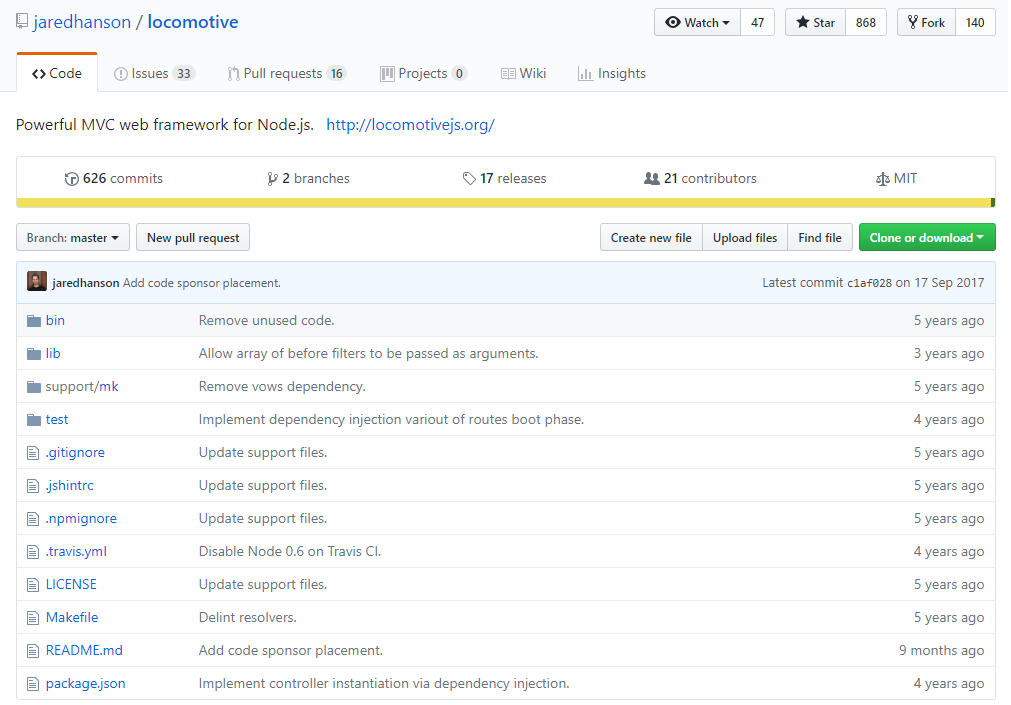
\includegraphics[width=\textwidth,height=\textheight,keepaspectratio]{locomotive.png} 
      \caption{Strona projektu Locomotive w serwisie Github \newline źródło: https://github.com/jaredhanson/locomotive/}
    \end{figure}
    Dla porównania framework Koa posiada 21568 gwiazdek oraz był aktualizowany w dniu pisania pracu (dane na dzień 06.06.2018).
    Możemy wieć założyć że jest wciąż popularny oraz utrzymywany.
    \begin{figure}[!hb]
      \centering
      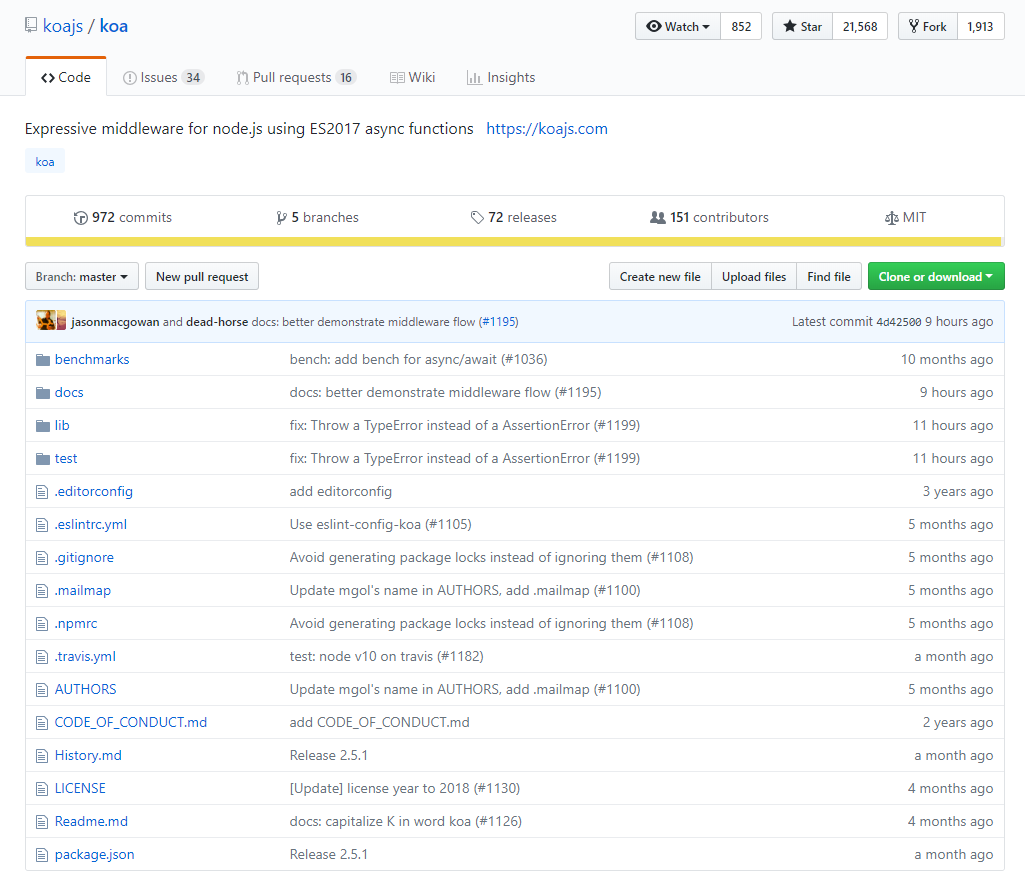
\includegraphics[width=\textwidth,height=\textheight,keepaspectratio]{koa.png} 
      \caption{Strona projektu Koa w serwisie Github \newline źródło: https://github.com/koajs/koa/}
    \end{figure}

  \section{Wybrane frameworki}
    Ilość dostępnych narzędzi nie pozwala niestety na porównanie wszystkich rozwiązań.
    W związku z czym zdecydowałem się przeanalizować w pracy 3 wybrane - Express, Sails oraz Meteor.

    \subsection{Express}
      Express wybrałem ze wzgłedu na jego ogromną popularność.
      Repozytorium projektu posiada prawie 40000 gwiazdek w serwisie Github oraz jest najpopularniejszy ze wszystkich frameworków w serwisie Stackoverflow (dane na dzień 06.06.2018).
      Ze wszystkich konkurencyjnych rozwiązań jest najpopularniej wymienianą technologią w ofertach pracy.
      Został wybrany aby sprawdzić czy wiodące rozwiązanie jest słusznie liderem na rynku.
      \begin{figure}[!hb]
        \centering
        
\includegraphics[width=\textwidth,height=\textheight,keepaspectratio]{express.png} 
        \caption{Strona projektu Express w serwisie Github \newline źródło: https://github.com/expressjs/express}
      \end{figure}

    \subsection{Sails}
      Sails został wybrany ze wzgłędu na wyjątkowo niski próg wejścia.
      Framework dostarcza nam gotowy szkielet aplikacji, który musimy dostosować pod nasze wymagania.
      Nie zyskał on jeszcze tak dużej popularności jak pozostałe rozwiązania, jednak dzięki prostocie zbiera on coraz więcej fanów.
      Jego użytkownicy podkreślają skalowalność, szybkość oraz uzyskaną produktywność jako największe jego zalety.
      Repozytorium projektu posiada prawie 20000 gwiazdek w serwisie Github (dane na dzień 06.06.2018).
      \begin{figure}[!hb]
        \centering
        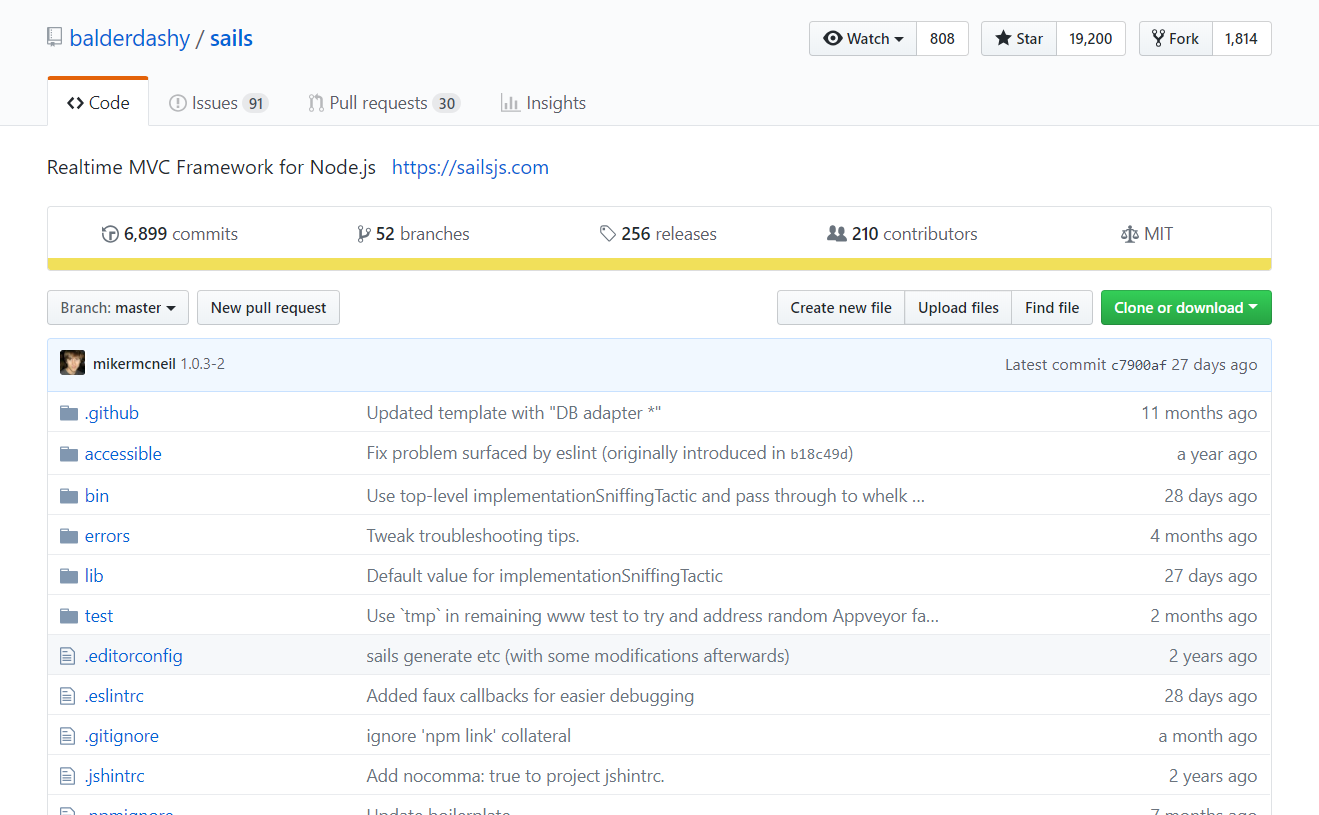
\includegraphics[width=\textwidth,height=\textheight,keepaspectratio]{sails.png} 
        \caption{Strona projektu Sails w serwisie Github \newline źródło: https://github.com/balderdashy/sails}
      \end{figure}

    \subsection{Meteor}
      Meteor wybrałem ponieważ mimo odcięcia się od tradycyjnego środowiska technologii Node.js, cieszy się on dużą popularnością oraz dostarcza nam możliwość wytwarzania jednocześnie częsci backendowej, frontendowej a nawet aplikacji mobilnych przy użyciu jednej bazy kodu.
      Framewok wprowadza wiele własnych narzędzi (np. własnego menadżera zależności, któremu w czystym Node.js odpowiada narzędzie Npm) oraz gotowych modułów zarówno widoku jak i logiki pozwalając na efektywniejsze wytwarzanie gotowego produktu.
      Repozytorium projektu posiada blisko 40000 gwiadek w serwisie Github (dane na dzień 06.06.2018).
      Popularność Meteor'a jest więc równa popularności frameworku Express, mimo że jest on od niego 2 lata młodszy.
      \begin{figure}[!hb]
        \centering
        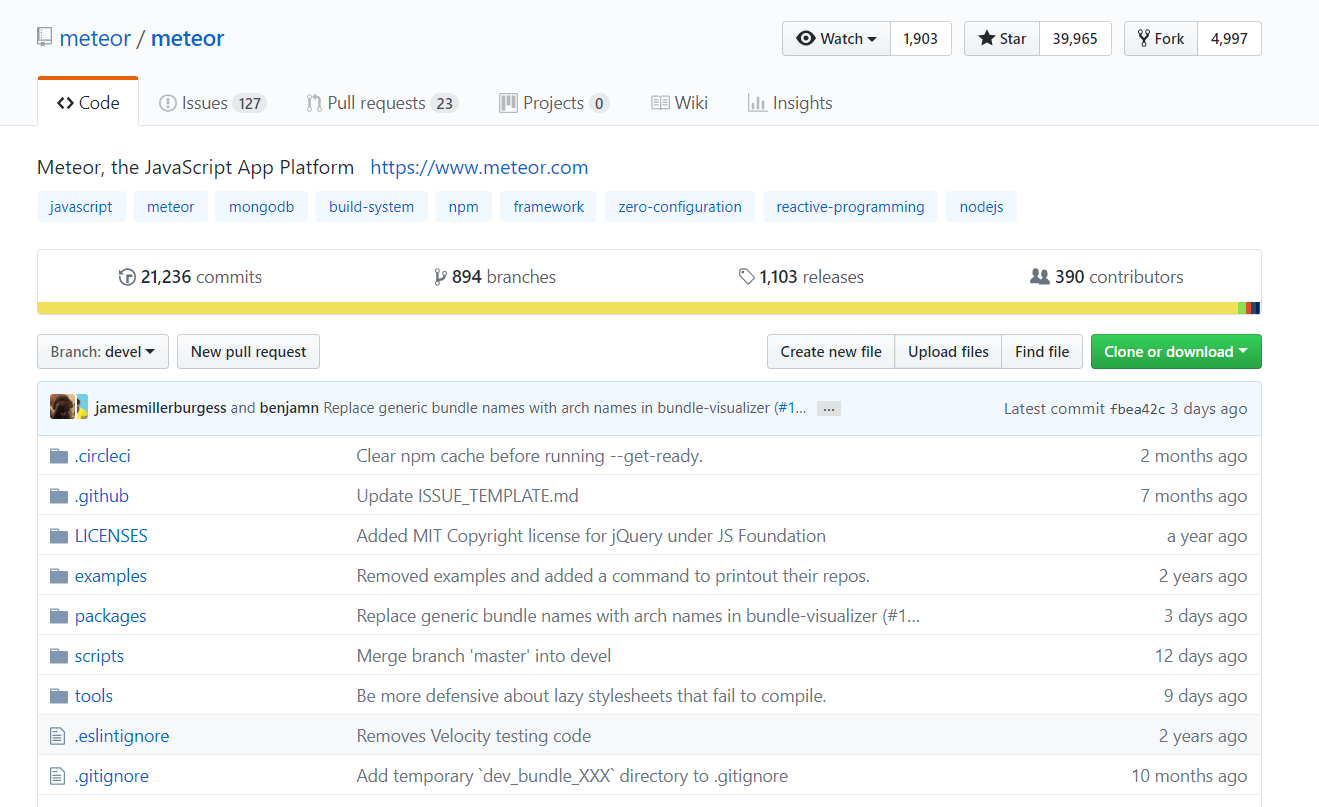
\includegraphics[width=\textwidth,height=\textheight,keepaspectratio]{meteor.png} 
        \caption{Strona projektu Meteor w serwisie Github \newline źródło: https://github.com/meteor/meteor}
      \end{figure}
  
  \section{Alternatywne rozwiązania}
    Rozdział opisuje alternatywne rozwiązania, które zostały wzięte pod uwagę podczas etapu poszukiwania.

    \subsection{Hapi}
    Zaprojektowany do wytwarzania nowoczenych serwisów stron internetowych.
    Posiada wiele zdefiniowanych reużywalnych modułów (walidacja, cache, autentykacja) wymagających tylko minimalnej konfiguracji.
    Pozwala on na zminimalizowanie budowy infrastruktury projektu, na korzyść skupienia się na tworzeniu logiki oraz funkcjonalności.

    \subsection{Koa}
    Stworzony przez twórców frameworka Express.
    Dostarcza możliwość wytwarzania częsci api serwisów.
    Po pierwszych prezentacjach Koa została przyjęta bardzo pozytywnie pozwalając na zminimalizowanie ilości pracy potrzebną na wytowrzenie produktu przy użyciu Express'a.
    Narzędzie jest jednak ciągle w fazie silnego rozwoju i nie dostarcza jeszcze tak szerokich jak Express możliwości.
    Z pewnością jest dla niego dobrą alternatywą w przypadku nieskomplikowanych serwisów.

    \subsection{Loopback}
    Framework fullstack'owy, zbudowany do tworzenia aplikacji mobilnych (systemy iOS oreaz Android) oraz aplikacji webowych wymagając bardzo niewielkich nakładów kodu.
    Do działania wykorzystuje Express.
    Dzięki narzędzią takim jak IBM API Connect możemy wytwarząć kod przy użyciu graficznego interfejsu.

\chapter{Kryteria oceny}

  \section{Skala oraz wagi ocen}
    Rozdział opisuje jakie parametry frameworków zostały przeanalizowane i skonfrontowane ze sobą.
    Frameworki zostały ocenione w skali od 1 do 3 pod kątem każdego z nich.
    Każdy z parametrów otrzymał wagę w skali od 1 do 3.
    Wagi oznaczają wpływ danego parametru na ocene podsumowującą.
    Końcowe oceny zostały wyliczone ze wzoru:
    \newline
    \newline
    \[\text{\Large$O = \frac{\sum_{i=1}^{n} p_{i} * w_{i}}{sw}$}\]
    \newline
    gdzie:
    \begin{description}
      \item[O] - ocena końcowa
      \item[n] - ilość parametrów
      \item[p] - ocena parametru
      \item[w] - waga parametru
	    \item[sw] - suma wag parametrów
    \end{description}
    Maksymalna ocena do uzyskania to 3.

  \section{Parametry}

    \subsection{Popularność}
      \begin{description}
        \item Waga: 3
      \end{description}
      Popularność jest wskaźnikiem, który niesie wiele infromacji na temat badanego frameworka.
      W najprostrzy sposób możemy ją sprawdzić za pomocą Google trends, w przypadku narzedzi open source przy użyciu statystyk repozytorium, a w przypadku pozostałych poprzez serwisy takie jak Stackoverflow.
      Dzięki popularności możemy wywnioskować wielokość społeczności jaka jest zainteresowana danym narzedziem.
      Wiąże się to z możliwym wsparciem, wartością rynkową oraz szerokością możliwych zastosowań jakie wspiera.
      Oczywistym jest że jeśli narzędzie posiada ogromną popularność zostało sprawdzone w dużej ilośći przypadków, a jeśli potrafi im sprostać umiejętności sprawnego posługiwania się nim stają się cenniejsze.

    \subsection{Rozmiar}
      \begin{description}
        \item Waga: 1
      \end{description}
      Rozmiar frameworku ma bezpośredni wpływ na rozmiar naszego końcowego produktu.
      Najbardziej pożądane jest aby narzędzie zajmowało jak najmniej miejsca.
      W celu zminimalizowania rozmiaru naszego produktu możemy użyć bundlerów takich jak np. webpack, które sprawią że do końcowego produktu zostanie załączona wyłącznie taka funkcjonalność biblioteki którą rzeczywiście wykorzystujemy.
      Warto o tym pamiętać w przypadku użycia dużych narzędzi dla prostych, niewymagających rozwiązań.
      Mimo takowej możliwości nie gwarantuje nam to zawsze małego rozmiaru produktu, dlatego rozmiar frameworku został wzięty pod uwagę.

    \subsection{Dokumentacja}
      \begin{description}
        \item Waga: 3
      \end{description}
      Nawet najbardziej użyteczne narzędzie nie mogłoby zaistnieć bez łatwo dostępnej, zrozumiale przekazanej dokumentacji.
      Jest ona niezbędna do przyswojenia proponowanych konceptów oraz obycia się z wybranym rozwiązaniem.
      Ocena dokumentacji dotyczy jej dostępności, szczegółowości oraz zrozumiałości.

    \subsection{Próg wejścia}
      \begin{description}
        \item Waga: 1
      \end{description}
      Próg wejścia oznacza ilość zagadnień wymaganych w celu opanowania danego frameworka oraz ilość czasu jaki należy poświęcić na jego opanowanie w stopniu conajmniej podstawowym.
      Pożądane jest aby był on jak najniższy; aby narzędzie nadawało się do użycia przez osoby jak najsłabiej znające koncepty programowania czy budowy systemów, niemal że natychmiast po chwilowym zapoznaniu się z dokumentacja.
      Ocena progu wejścia została wystawiona na podstawie trudności oraz czasu poświęconego na zaznajomienie się z analizowanym narzędziem w stopniu umożliwiającym stworzenie funkcjonalności przedstawionej w opisanej pracy.

    \subsection{Warstwa widoku}
      \begin{description}
        \item Waga: 2
      \end{description}
      Parametr opisuje w jakim stopniu badany framework zapewnia obsluge warstwy widoku wytwarzanej aplikacji.
      Możemy oczekiwać wielu możliwości obsługi warstwy widoku.
      Wydawać by się mogło, że najlepszą możliwością byłoby gdyby framework kompletnie integrował warstwe widoku z warstwą danych dostarczając określone, proste metody wzajemnego mapowania.
      Kompletnie nie porządane z koleji jest, aby do obsługi oraz integracji z warstwą widoku wytwarzanego produktu było wymagane użycie zewnętrznego, dodatkowego narzędzia.
      Ocena została wystawiona na podstawie możliwości jakie oferują analizowane frameworki bez użycia dodatkowych narzędzi.

    \subsection{Warstwa bazy danych}
      \begin{description}
        \item Waga: 2
      \end{description}
      Podobnie jak parametr warstwy widoku, parametr ten opisuje możliwość integracji frameworka z bazą danych.
      Najmniej pożądanym zachowaniem jest kiedy moduł obsługi bazy danych należy w całości dołączyć do rozwiązania, natomiast najbardziej pożądanym aby framework w pełni posiadał zaimplementowaną integracje przy użyciu np. komponentu DAO.
      Ocena została wystawiona na podstawie możliwości jakie oferują analizowane narzędzia bez użycia dodatkowych narzędzi.

    \subsection{Ilość kodu}
      \begin{description}
        \item Waga: 2
      \end{description}
      Parametr opisuje ilość kodu potrzebnego do napisania aby otrzymać ideantyczną funkcjonalność w analizowanych środowiskach.
      Ilość kodu pisanego przy użyciu tego samego języka oraz jego standardu z zachowaniem odpowiednich praktych może zostać przełożony na ilość pracy, a co za tym idzie czasu jaki należy poświęcić do osiągnięcia obranego celu.
      Napisany kod musi być zgodny ze stosowanymi, ogólnie uznanymi praktykami programistycznymi dla danych środowisk.
      Parametr opisuje również najważniejsze feature's frameworków, które umożliwiają zmiejszenie ilości wymaganego kodu.
      Oceny zostały wystawione na podstawie porównania uzyskanych wyników dla analizowanych narzędzi.

    \subsection{Rozszerzalność}
      \begin{description}
        \item Waga: 3
      \end{description}
      Parametry rozszerzalności dotyczy możliwości rozszerzania istniejącego kodu o nowe oraz łatwości zmian istniejących funkcjonalności.
      Rozszerzalny kod charakteryzuje czytelny, jasny sposób zapisu, reużywalność istniejących już modułów, klas lub metod oraz odporność na zmiany częsci kodu bez wprowadzania regresji w pozostałych.
      Taki sposób pisania gwarantuje łatwiejsze zarządzanie oraz utrzymanie kodu.
      Dobry framework powinien wymuszać na programiście pisanie modularnego, rozszerzalnego kodu lub przynajmniej dostarczać przejrzyste sposoby na jego osiągnięcie.
      Jako że zbadanie rozszerzalności kodu jest trudne i jego możliwość lub jej brak może zostać zauważona po odpowiednim rozwoju aplikacji ocena tego zagadnienia została wystawiona na podstawie tworzenia przykładowej funkcjonalności do analizy pozostałych parametrów.

    \subsection{Testowanie}
      \begin{description}
        \item Waga: 2
      \end{description}
      Parametr opisuje stopień trudności wytworzenia testów automatycznych kodu dla danego środowiska.
      Stworzenie automatycznych testów pozwala nam w najszybszy dostępny sposób sprawdzić czy testowane rozwiązanie zachowuje się zgodnie z założonymi oczekiwaniami.
      Znacznie skraca to czas wytwarzania oprogramowania dzięki natychmiastowej diagnostyce oraz możliwości wyeliminowania powstałych błedów.
      Analizowany framework powinien dostarczać metody łatwego tworzenia testów automatycznych lub bezproblemową integracje w przypadku użycia zewnętrznego narzędzia.
      Ocena została wystawiona na podstawie stworzenia testów automatycznych dla analizownych środowiska przy użyciu dostarczonych przez framework możliwości.

    \subsection{Testy sprawnościowe}
      \begin{description}
        \item Waga: 3
      \end{description}
      Parametr opisuje ilość przetworzonych zapytań w ciągu określonego czasu.
      Kolejne zapytania zostają wysłane dopiero po otrzymaniu odpowiedzi na poprzednie.
      Możemy w ten sposób sprawdzić jak sprawnie aplikacja wykonana w konkretnym środowisku jest w stanie odpowiadać na nieustające zapytania końcowego użytkownika.
      Zapytania zostały dobranego dla różnych przypadków użycia:
      \begin{description}
        \item Autoryzacja - uzyskanie autoryzacji na zapytanie zawierające login oraz hasło użytkownika
        \item Zapis danych użytkownika - zapisanie danych tekstowych użytkownika w bazie danych
        \item Proste zapytanie o zasób - uzyskanie dostępu do zasobu tekstowego z bazy danych przez użytkownika
        \item Zapytanie o zasób - uzyskanie dostępu do zasobu multimedialnego (pliku w formacie png) z serwera
        \item Streaming multimediów - uzyskanie dostępu do streamu multimedialnego (w formacie avi) z serwera
      \end{description}
      Okresy czasu dla których zostały wykonane testy to:
      \begin{description}
        \item krótki - 2 sekundy
        \item średni - 10 sekund
        \item długi - 30 sekund
      \end{description}
      Oceny zostały wystawione na podstawie porównania uzyskanych wyników dla analizowanych narzędzi.
      
    \subsection{Testy obciążeniowe}
      \begin{description}
        \item Waga: 3
      \end{description}
      Parametr opisuje czas potrzebny na przetworzenie różnych ilości równolegle przycho-dzących zapytań, symulując prace serwera przy obciążeniu od wielu użytkowników w tym samym czasie.
      Zapytania zostały wysłane w tym samym momencie i został zmierzony czas po którym uzyskano odpowiedź na wszystkie z nich.
      Zapytania zostały dobrane dla następujących przypadków użycia:
      \begin{description}
        \item Autoryzacja - uzyskanie autoryzacji na zapytanie zawierające login oraz hasło użytkownika
        \item Zapis danych użytkownika - zapisanie danych tekstowych użytkownika w bazie danych
        \item Proste zapytanie o zasób - uzyskanie dostępu do zasobu tekstowego z bazy danych przez użytkownika
        \item Zapytanie o zasób - uzyskanie dostępu do zasobu multimedialnego (pliku w formacie png) z serwera
        \item Streaming multimediów - uzyskanie dostępu do streamu multimedialnego (w formacie avi) z serwera
      \end{description}
      Ilości wysłanych równolegle zapytań to:
      \begin{description}
        \item mała - 5 zapytań
        \item średnia - 30 zapytań
        \item duża - 150 zapytań
      \end{description}
      Oceny zostały wystawione na podstawie porównania uzyskanych wyników dla analizowanych narzędzi.

\chapter{Opis wybranych rozwiązań}

  \section{Express}
    \begin{figure}[!hb]
      \centering
      
\includegraphics[width=\textwidth,height=\textheight,keepaspectratio]{logo_express.png} 
      \caption{Logo projektu Express \newline źródło: https://expressjs.com/}
    \end{figure}
    Express jest najbardziej popularnym frameworkiem technologii Node.js.
    Często jest używany również jako podstawa na której opierają się inne frameworki tej technologii.
    Został stworzony do tworzenia serwerów oferujących między innymi możliwości:
    \begin{itemize}
      \item obsługi routingu zapytań protokołu http
      \item integracji z silnikami prezentacji danych poprzez użycie szablonów
      \item tworzenia narzędzi sieciowych do zarządzania innymi serwerami
      \item tworzenie pośredniczących mikroserwisów
    \end{itemize} 
    Sama podstawa frameworka jest utrzymywana w jak najbardziej minimalistycznej formie.
    Wspiera on polityke tworzenia modułów obsługujących daną funkcjonalność przez społeczeństwo deweloperów.
    Dzięki repozytorium Npm w łatwy sposób możemy znaleźć rozwiązanie gotowe na praktycznie każdy problem.
    Powstaje jednak kwestia wyboru właściwego, stworzonego w najbardziej optymalnie.
    Wiele z modółów zostaje zatwierdzonych przez grupe deweloperów tworzących framework jako sprawdzone, co zwiększa zaufanie oraz pomaga promować najlepsze rozwiązania.
    Express pozwala pisać aplikacje w bardzo elastyczny sposób, nie narzucając jednej słusznej drogi.
    Pozwala na tworzenie dowolnej architektury własnego serwera.
    Został stworzony w 2010 roku, wydany na licencji MIT przez firme StrongLoop.
    Do analizy została użyta wersja 4.16.3.

   \section{Sails}
    \begin{figure}[!hb]
      \centering
      
\includegraphics[width=\textwidth,height=\textheight,keepaspectratio]{logo_sails.png} 
      \caption{Logo projektu Sails \newline źródło: https://sailsjs.com/}
    \end{figure}
    Sails jest to framework aplikacji webowych działający w architekturze MVC (Model-View-Controller).
    Inspiracją do jego powstanie był framework Ruby on Rails dla języka Ruby, a do jego napisania został wykorzystany Express.
    Pozwala on na budowe:
     \begin{itemize}
      \item serwisów rest API
      \item aplikacji single-page 
      \item aplikacji czasu rzeczywistego
    \end{itemize} 
    Sails prezentuje ściśle określoną architekturę projektu zdejmując z programistów obowiązek jej tworzenia.
    Jednym z podstawowych założeń tego narzędzia jest konfigurowalność dostarczonych, gotowych komponentów ponad pisanie własnych.
    Narzędzie wykorzystuje skonfigurowane pliki w języku javaScript i generuje na ich podstawie gotowy produkt.
    Został stworzony w 2012 roku, wydany na licencji MIT przez firme The Sails Company.
    Do analizy została użyta wersja 1.0.2.

  \section{Meteor}
    \begin{figure}[!hb]
      \centering
      
\includegraphics[width=\textwidth,height=\textheight,keepaspectratio]{logo_meteor.png} 
      \caption{Logo projektu Meteor \newline źródło: https://www.meteor.com/}
    \end{figure}
    Meteor wyróżnia przedewszystkim, fakt że jest frameworkiem izomorficznym. 
    Jeden kod aplikacji działa zarówno po stronie klienta jak i serwera.
    Służy do szybkiego tworzenia wielo-platformowych aplikacji (Android, iOS, web).
    Platforma odeszła od tradycyjnych narzędzi środowiska Node.js i stworzyła własny ekosystem budowania projektów czy menadzera modułów.
    Architektura komunikacji między warstwa frontendu, a backendu nie korzysta z zapytań http, a z subskrypcji modelu danych poprzez web sockety.
    Został stworzony z myśłą o aplikacjach:
    \begin{itemize}
      \item single-page 
      \item czasu rzeczywistego
      \item wymagających wysokiej synchronizacji danych
    \end{itemize} 
    Framework wymusza na programiście korzystanie z paradygmatu reaktywnego.
    Skupia się on na reagowaniu na zmiany obserwowanego modelu danych.
    Został stworzony w 2012 roku, wydany na licencji MIT przez firme Meteor Development Group.
    Do analizy została użyta wersja 1.9.2.

\chapter{Analiza porównawcza}

  \section{Express}
    \subsection{Popularność}
      Na portalu Github możemy zobaczyć, że framework posiada prawie 40000 gwiazdek.
      Na portalu Stackoverflow znajduję się prawie 45000 wątków dotyczących tej technologii.
      Obsługa narzędzia jest również najczęsciej poszukiwaną umiejętnością na rynku pracy w technologii Node.js.
      (dane na dzień 28.06.2018).

    \subsection{Rozmiar}
      Framework możemy zainstalować używając podstawowego menadzera zależności środowiska Node.js - Npm, używając komendy:
      \begin{lstlisting}[language=bash,numbers=none]
        npm install express
      \end{lstlisting}
      Po instalacji zostanie utworzony folder node\_modules zawierający tylko podstawowe komponenty frameworka, ważący 2.19 mb.
      Aby jednak w jak najbardziej wydajny sposób osiągnąć zadaną funkcjonalność należy zainstalować pare brakujących modułów.
      Po zainstalowaniu:
      \begin{itemize}
        \item Mongoose - obsługa bazy danych mongoDB
        \item Passport - autentykacjia użytkownika
        \item Bcrypt - przechowywanie haseł
        \item Helmet - bezpieczeństwo zapytań http
        \item Body-parser - obsługa ciał zapytań http
        \item Joi - walidacja zapytań http
        \item Express-session, Cookie-parser, Connect-flash - obsługa sesji oraz ciasteczek
        \item Mocha, Supertest, Chai oraz Cheerio - testy 
      \end{itemize} 
      Waga zwiększa się do 18.0 mb.
      Po stworzeniu plików źródełowych kompletna aplikacjia waży 18.1 mb.
      Można więc uznać to za wagę wyjściową, która powinna być wzięta przy analizie.

    \subsection{Dokumentacja}
      Strona dokumentacji jest dostępna na stronie https://expressjs.com/en/api.html.
      Jest utrzymana w bardzo prostym, minimalistycznym designie, co sprawia że łatwo się po niej poruszać oraz wyszukiwać informacje.
      Posiada opisy pól i metod z podstawowego modułu Express, oraz krótkie, nieskomplikowane przykłady użycia.
      Dla niektórych zagadniej (na przykład template rednering) znajduje się tylko szczątkowa ilość informacji.
      Możemy znaleźć również dokumentacje pozostałych modułów utrzymywanych lub także polecanych przez zespół stojący za frameworkiem dla poszczególnych funkcjonalności.
      Na stronie brakuje wskazówek odnośnie polecanych modeli architektury projektu, które byłyby przydatne dla początkujących użytkowników.
      \begin{figure}[!hb]
        \centering
        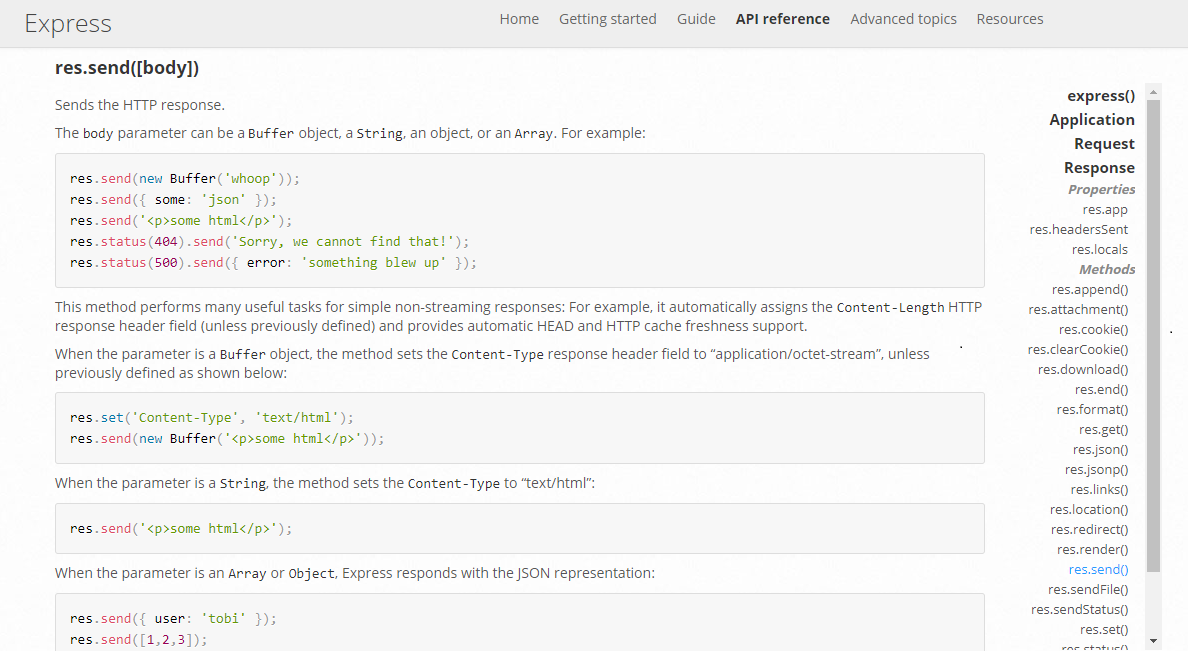
\includegraphics[width=\textwidth,height=\textheight,keepaspectratio]{doc_express.png} 
        \caption{Dokumentacja projektu Express \newline źródło: https://expressjs.com/en/api.html}
      \end{figure}

    \subsection{Próg wejścia}
      Do stworzenia prostej aplikacji framework wydaje się wymagać tylko znajomości języka javaScript.
      Wymagania rosną natomiast wraz z wielkością projektu.
      W celu uzyskania wielu z podstawowych funkcjonalności (poza routingiem oraz middlewares, które zapewnia Express) należy użyć zewnętrznych bibliotek, co wymaga wcześniejszego ich opanowania. 
      Aby utrzymać kod w należytym ładzie należy również posiadać odpowiednie doświadczenie programistyczne.
      Wymagania te nie są jednak wygórowane i nie powinny być przeszkodą po krótkim zapozaniu się ze środowiskiem.

    \subsection{Warstwa widoku}
      W celu opracowania widoku aplikacji możemy wybrać między skorzystaniem z zewnętrznego rozwiazania (np. bibliotek frontendowych Angular, Vue, React) lub użyciem wspieranego przez Express renderingu po stronie serwera przy użyciu szablonów (ang. server side template rendering).
      Technika ta polega na stworzeniu odpowiednich reużywalnych wzorców widoków stron przy użyciu wybranego silnika (np. Pug lub Ejs) oraz zmiany renderowanych wartości wzorca zależnie od stanu aplikacji. 
      Każdy z silników posiada specyficzną składnie, dzięki której zamienia otrzymane wartości na strone html.
      Do opracowania rozwiązania zdecydowałem się na skorzystanie z metod renderowania po stronie serwera z użyciem silnika Ejs.

    \subsection{Warstwa bazy danych}
      Framework Express nie dostarcza żadnych integracji z bazą danych. 
      W celu jej zapewnienia należy skorzystać z zewnętrznego narzędzia.
      Dla baz danych typu nosql (np. MongoDb) najpopularniejszym rozwiązaniem jest biblioteka mongoose.
      Daje ona wysokopoziomowy interfejs na odpowiednie metody wybranych baz danych oraz przekształca rekordy przy użyciu ODM (object document mapping).
      Dla baz danych typu sql (np. Postgres) najpopularniejszym roziązaniem jest biblioteka Sequelize.
      Pozwala ona na zaprzestanie używania języka sql na rzecz wysokopoziomowyh metod oraz dostęp do rekordów przy użyciu ORM (object relational mapping).
      Do oprawcowania aplikacji zdecydowałem się skorzystać z MongoDB oraz modułu Mongoose.

    \subsection{Ilość kodu}
      Ilość wytworzonych lini kodu to około 500. 
      Najważniejszymi cechami frameworka, które przyśpieszają proces wytwórczy są użycie middlewares oraz routingu.
      Pierwszy z nich pozwala na ułożenie pewnego przepływu funkcji przy obsłudzę przychodzacych zapytań.
      Możemy zapewnić ciąg usług jakie zostaną wywołane w odpowiedniej kolejności (np. logowanie, autentykacjia).
      Drugi pozwala na wysokopoziomowe zarządzanie funkcjami obsługującymi przychodzące zapytania http.
      Dopasowywane są one do żadanego adresu.
      Te features pozwalają na skupieniu się na tworzeniu głównie warstwy biznesowej aplikacji bez potrzeby bezpośredniego zarządzania warstwą komunikacji, skutecznie zmiejszając wymagany nakład pracy.

    \subsection{Rozszerzalność}
      Jako że środowisko Express nie narzuca absolutnie żadnej sztywnej architektury wytwarzanego projektu rozszerzalność jaką uda nam się uzyskać zależy tylko od naszego własnego doświadczenia i umiejętności.
      Nie wątpliwie jest to problem dla nowych programistów oraz przy napotkaniu nowego projektu o nieznanej strukturze.
      Aby utrzymać kod czytelnym i klarownym wiele źródeł proponuje skorzystać przy budowie projektu ze wzorca MVC.
      Projekt podzielić wówczas na:
      \begin{itemize}
        \item model - reprezentacja stanu aplikacji
        \item widoki - szablony widoków
        \item kontrolery - obsługa routerów oraz ich logiki
        \item middlewares - obsługa middlewares (komponentów wspierających dane funkcjonalności)
        \item public - statyczne pliki jak multimedia czy style
        \item test - skrypty testujące
        \item helpers - funkcjonalność współdzielona między różnymi częściami projektu
      \end{itemize}
      Zapewni to odpowiednie rozgraniczenie między odpowiedzialnościami poszczególnych części dzięki czemu osiągniemy szczątkowe zapewnienie o łatwości rozszerzalności aplikacji. 
      
    \subsection{Testowanie}
      Express nie dostarcza nam wraz z frameworkiem metod testujących wytwarzaną aplikacje. 
      Najbardziej popularną biblioteką do testów tego narzędzia jest Mocha.
      Jest to biblioteka służąca do pisania każdego rodzaju przypadków testowych.
      Należy określić porządane efekty oraz sposób jak mają zostać uzyskane i zapakować je w test suits oraz test cases.
      Po użyciu narzędzia otrzymano wyniki:
      \begin{figure}[!hb]
        \centering
        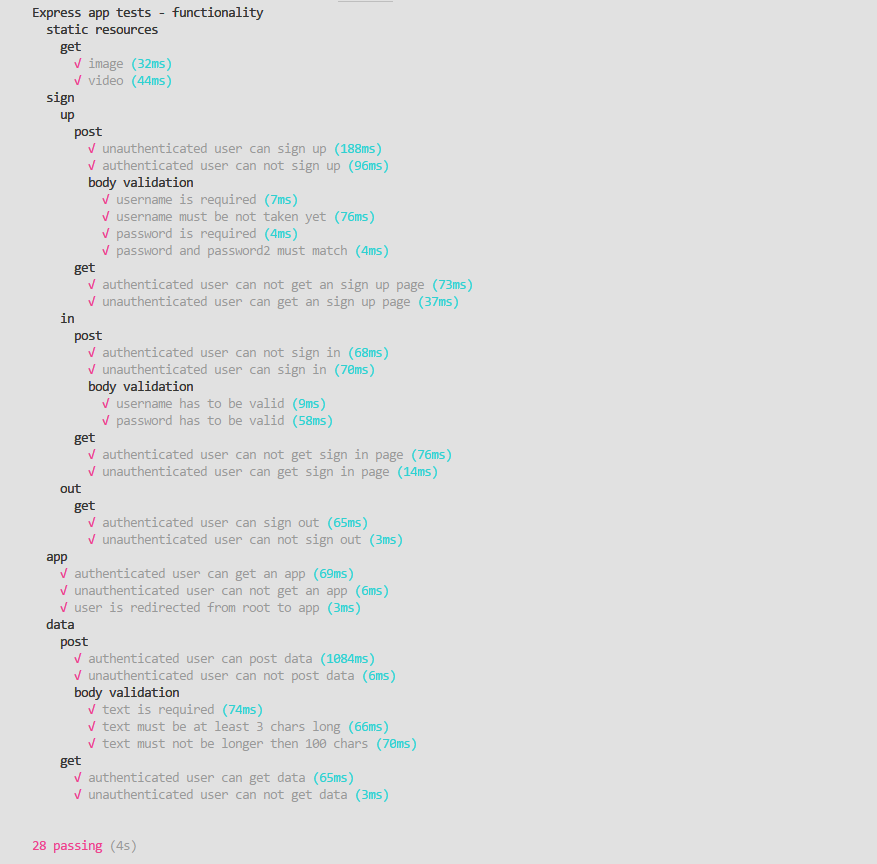
\includegraphics[width=\textwidth,height=\textheight,keepaspectratio]{test_express.png} 
        \caption{Testy frameworka Express przy użyciu biblioteki Mocha \newline źródło: opracowanie własne}
      \end{figure}

    \subsection{Testy sprawnościowe}
      Testy zostały przeprowadzone przy użyciu biblioteki Mocha, Supertest oraz Chai.
      Podane wyniki reprezentują ilość przetworzonych zapytań w określonym czasie dla wybranych funkcjonalności.
      \newline
      \newline
      \newline
      \newline
      \newline
      \newline
          \begin{tabular}{|c|c|c|c|c|c|p{2.2cm}}
            \hline
            \parbox{2.2cm}{Okres czasu} & 
            \parbox{2.2cm}{Autoryzacja} & 
            \parbox{2.2cm}{Zapis danych tekstowych użytkownika} & 
            \parbox{2.2cm}{Zapytanie o zasób tekstowy użytkownika} & \parbox{2.2cm}{Zapytanie o zasób obraz} & 
            \parbox{2.2cm}{Streaming multimediów video} \\
            \hline
            2 sekundy & 396 & 144 & 420 & 463 & 147 \\
            \hline
            10 sekund & 2326 & 1501 & 1692 & 2933 & 696 \\
            \hline
            30 sekund & 6126 & 3103 & 4019 & 9143 & 1857 \\
            \hline
            \parbox{2.2cm}{Średnia ilość dla 1 sekundy} & 210 & 113 & 146 & 299 & 64 \\
            \hline
          \end{tabular}
      \newline
      \newline
      \newline
      \newline
    \subsection{Testy obciążeniowe}
      Testy zostały przeprowadzone przy użyciu biblioteki Mocha, Supertest oraz Chai.
      Podane wyniki reprezentują czas otrzymania odpowiedzi dla odpowiednich ilości zapytań w sekundach dla wybranych funkcjonalności.
      \smallskip
        \begin{center}
          \begin{tabular}{ | c | c | c | c | c | c | }
            \hline
            Ilości wysłanych równolegle zapytań & Autoryzacja & Zapis danych tekstowych użytkownika & Zapytanie o zasób tekstowy użytkownika & Zapytanie o zasób obraz & Streaming multimediów video \\
            \hline
            5 jednocześnie wysłanych zapytań & 1.174 & 0.02 & 0.015 & 0.002 & 0.003 \\
            \hline
            30 jednocześnie wysłanych zapytań & 1.552 & 0.107 & 0.063 & 0.013 & 0.014 \\
            \hline
            150 jednocześnie wysłanych zapytań & 7.799 & 0.407 & 0.282 & 0.066 & 0.069 \\
            \hline
            Średni czas dla 1 zapytania & 0.056 & 0.02 & 0.02 & 0.0004 & 0.0004 \\
            \hline
          \end{tabular}
        \end{center}
      \bigskip\medskip

  \section{Sails}

    \subsection{Popularność}
      Na portalu Github możemy zobaczyć, że framework posiada prawie 20000 gwiazdek.
      Na portalu Stackoverflow znajduję się około 6000 wątków dotyczących tej technologii.
      (dane na dzień 28.06.2018).

    \subsection{Rozmiar}
      Do pobrania frameworka jako aplikacji konsolowej używamy polecenia:
      \begin{lstlisting}[language=bash,numbers=none]
        npm install sails -g
      \end{lstlisting}
      Po zainstalowaniu do stworzenia szkieletu projektu używamy:
      \begin{lstlisting}[language=bash,numbers=none]
        sails new [nazwa aplikacji]
      \end{lstlisting}
      Stworzony projekt (wraz z pobranymi zależnościami) waży 176 mb.
      Po napisaniu kodów źródłowych waga jest równa 177 mb.
      Można więc uznać to za wagę wyjściową, która powinna być wzięta przy analizie.

    \subsection{Dokumentacja}
      Strona dokumentacji jest dostępna na stronie https://sailsjs.com/documentation.
      Możemy tam znaleźć zarówno ogólne, użyteczne przy gruntownym rozeznaniu oraz szczegółowe opisy poszczególnych części frameworka.
      W czytelny i łatwy do odszukania sposób mamy dostęp do wydawać by się mogło każdego szczególu na temat tego środowiska.
      Dokumentacja jest napisana zrozumiałym ale nie upraszczają-cym językiem oraz posiada załączone zrzuty i odnośniki do przykładowych kodów źródłowych.
      Dostępne są opisy struktury architektury, wyjaśnienia konceptów oraz szczegółowe opisy użytecznych feature'ów.
      \begin{figure}[!hb]
        \centering
        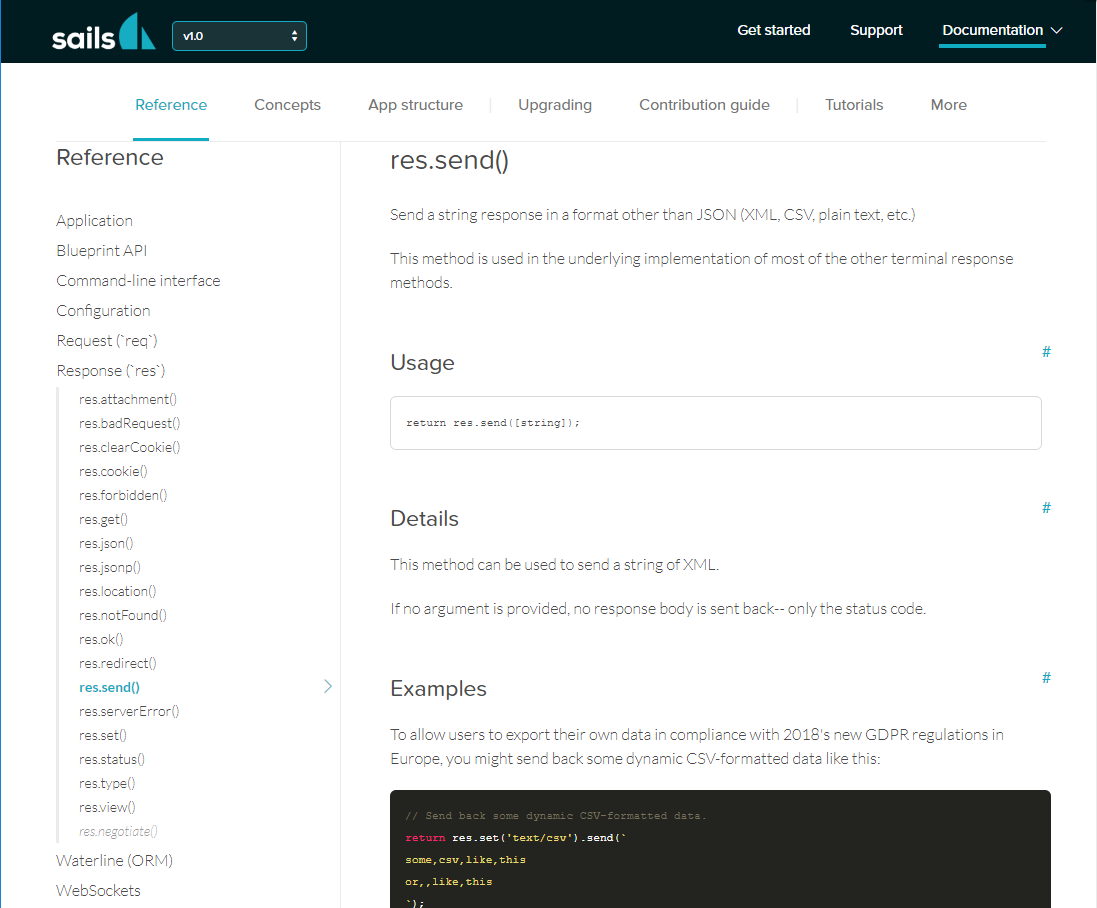
\includegraphics[width=\textwidth,height=\textheight,keepaspectratio]{doc_sails.png} 
        \caption{Dokumentacja projektu Sails \newline źródło: https://sailsjs.com/documentation}
      \end{figure}

    \subsection{Próg wejścia}
      Sails jest wyjątkowo prosty w obsłudze.
      Do stworzenia podstawy projektu używamy jednego polecenia, a dalsza praca polega na pisaniu logiki na wzór już istniejącej.
      Ponadto dzięki przystępnie napisanej dokumentacji nie istnieją problemy nawet z rozwiązaniem bardziej skomplikowanych zagadnień.
      Wiele wymagań możemy pokryć już w procesie konfiguracji bez potrzeby pisania kodu.
      Dzięki sztywnej, z góry określonej strukturze aplikacji, mimo wielu możliwości łatwo jest zrozumieć sposób pracy zarówno przy tworzniu nowego jak i wdrażania w istniejący projekt. 

    \subsection{Warstwa widoku}
      Jako że Sails został stworzony przy użyciu Express warstwa widoku rządzi się dokładnie tymi samymi zasadami.
      Możemy wybrać między skorzystaniem z zewnętrznego rozwiazania (np. bibliotek frontendowych Angular, Vue, React) lub użyciem renderingu po stronie serwera przy użyciu szablonów (ang. server side template rendering).
      Domyślnie używanym przez Sails silnikiem jest Ejs, który zdecydowałem się wykorzystać przy tworzeniu przykładowej aplikacji.

    \subsection{Warstwa bazy danych}
      Do obsługi warstwy bazy danych Sails wykorzystuje biblioteke Waterline.
      Jest to biblioteka ORM dostarczająca zunifikowane API do obsługi między innymi MySQL, PostgreSQL czy MongoDB.
      Posiada ona wiele użytecznych feature'ów takich jak automatyczne replikacje, czy nawet populowanie między bazami danych w różnych technologiach. 
      W celu wybrania źródła danych nie musimy ustawiać dialektu, wystarczy tylko wskazać adres bazy.
      Domyślnie, na potrzeby dewelopmentu framework dostarcza baze danych Sails-disk, która symuluje działania realnej bazy danych.
      Nie powinna być ona używana jednak w środowisku produkcyjnym.

    \subsection{Ilość kodu}
      Ilość wytworzonych lini kodu to około 400.
      Są to jednak linie kodu bardziej skupione na konfiguracji wartości lub nieskomplikowanej logice w porównaniu z kodem aplikacji napisanej przy użyciu Express.
      Ponieważ framework został napisany przy użyciu narzędzia Express możemy korzystać ze wszystkich jego feature'ów min. middlewares.
      Sails zapewnia dodatkowo bardzo wiele możliwości.
      Najbardziej rozpoznawalną są blueprints, które pozwalają na automatyczne generowanie pełnej funkcjonalności rest api (wraz z interfejsem komunikacji oraz połączeniem z bazą danych) dla stworzonych modeli danych.
      Kolejnym dostępnym feature'em jest routing (pochodzący z Express) wzbogacony o automatyczne tworzenie końcówek http dla wytworzonych kontrolerów wedug ich scieżki w projekcie.
      Framework oferuje także nieskomplikowane w obsłudzę zarządzanie dostępem do zasobów aplikacji przez pollicies, działających na podstawie określonych kontrolerów dostępu.
      Poza wymienionymi mamy również dostęp do mniej skomplikowanych funkcjonalności jak walidacja zapytań, automatyczne tworzenie dokumentacji czy internacjonalizacja aplikacji.
      Każda funkcjonalność jest konfigurowana na podstawie osobnych plików konfiguracyjnych w postaci obiektów języka javaScript.
      Wszystko to sprawia, że możemy skupić się wyłącznie na pisaniu kodu biznesowego.

    \subsection{Rozszerzalność}
      Sails działa w sztywno określonej architekturze opartej na wzorcu MVC.
      Po stworzeniu szkieletu aplikacji jest ona podzielona na foldery:
      \begin{itemize}
        \item api, składające się z:
        \begin{itemize}
          \item controllers - obsluga przychodzących zapytań, interakcja z modelem
          \item helpers - współdzielona między komponentami funkcjonalność
          \item pollicies - zarządzanie dostępem do zasobów aplikacji
          \item models - struktura danych aplikacji
          \item responses - reużywalne szablony dla odpowiedzi aplikacji
        \end{itemize}
        \item assets - statyczne pliki serwisu jak multimedia czy style
        \item views - szablony widoków aplikacji
        \item tasks - funkcje oraz skrypty wywoływane dla różnych stanów aplikacji (np. Grunt lub Webpack)
        \item config - pliki konfigracyjne środowiska jak tłumaczenia, przełączniki, adresy baz danych
      \end{itemize}
      Wymuszenie sztywnego podziału gwarantuje szybkie odnalezienie się w nowych projektach oraz wskazuję droge do osiągnięcia zrozumiałego, czystego kodu.
      Dzięki konfigurowalności aplikacji jest ona również odporna na możliwe do szybkiego wprowadzenia zmiany.
      Projekty wytworzone narzędziem są dzięki temu łatwo utrzymywalne i rozszerzalne nawet przy braku dużego doświadczenia programistycznego. 

    \subsection{Testowanie}
      Sails nie dostarcza nam wraz z frameworkiem metod testujących wytwarzaną aplikacje. 
      Najbardziej popularną biblioteką do testów tego narzędzia jest Mocha.
      Jest to framework służący do pisania każdego rodzaju przypadków testowych.
      Należy określić porządane efekty oraz sposób jak mają zostać uzyskane i zapakować je w test suits oraz test cases.
      Po użyciu narzędzia otrzymano wyniki testów:
      \begin{figure}[!hb]
        \centering
        \includegraphics[width=\textwidth,height=\textheight,keepaspectratio]{test_Sails.png} 
        \caption{Testy frameworka Sails przy użyciu biblioteki Mocha \newline źródło: opracowanie własne}
      \end{figure}

    \subsection{Testy sprawnościowe}
      Testy zostały przeprowadzone przy użyciu biblioteki Mocha, Supertest oraz Chai.
      Podane wyniki reprezentują ilość przetworzonych zapytań w określonym czasie dla wybranych funkcjonalności.
      \smallskip
        \begin{center}
          \begin{tabular}{ | c | c | c | c | c | c | }
            \hline
            Okres czasu & Autoryzacja & Zapis danych tekstowych użytkownika & Zapytanie o zasób tekstowy użytkownika & Zapytanie o zasób obraz & Streaming multimediów video \\
            \hline
            2 sekundy & 210 & 210 & 243 & 280 & 127 \\
            \hline
            10 sekund & 1187 & 1036 & 1020 & 1499 & 627 \\
            \hline
            30 sekund & 2926 & 2336 & 2712 & 3992 & 1613 \\
            \hline
            Średnia ilość dla 1 sekundy & 103 & 85 & 95 & 137 & 56 \\
            \hline
          \end{tabular}
        \end{center}
      \bigskip\medskip

    \subsection{Testy obciążeniowe}
      Testy zostały przeprowadzone przy użyciu biblioteki Mocha, Supertest oraz Chai.
      Podane wyniki reprezentują czas otrzymania odpowiedzi dla odpowiednich ilości zapytań w sekundach dla wybranych funkcjonalności.
      \smallskip
        \begin{center}
          \begin{tabular}{ | c | c | c | c | c | c | }
            \hline
            Ilości wysłanych równolegle zapytań & Autoryzacja & Zapis danych tekstowych użytkownika & Zapytanie o zasób tekstowy użytkownika & Zapytanie o zasób obraz & Streaming multimediów video \\
            \hline
            5 jednocześnie wysłanych zapytań & 1.015 & 0.037 & 0.025 & 0.009 & 0.011 \\
            \hline
            30 jednocześnie wysłanych zapytań & 6.271 & 0.17 & 0.215 & 0.07 & 0.079 \\
            \hline
            150 jednocześnie wysłanych zapytań & 31.261 & 0.796 & 1.021 & 0.258 & 0.254 \\
            \hline
            Średni czas dla 1 zapytania & 0.208 & 0.005 & 0.007 & 0.002 & 0.002 \\
            \hline
          \end{tabular}
        \end{center}
      \bigskip\medskip

  \section{Meteor}

    \subsection{Popularność}
      Na portalu Github możemy zobaczyć, że framework posiada prawie 40000 gwiazdek.
      Na portalu Stackoverflow znajduję się około 28000 wątków dotyczących tej technologii.
      (dane na dzień 28.06.2018).

    \subsection{Rozmiar}
      Do pobrania frameworka jako aplikacji konsolowej dla systemu windows używamy menadzera Chocolatey, używając polecenia
      \begin{lstlisting}[language=bash,numbers=none]
        choco install meteor
      \end{lstlisting}
      Narzędzie waży 389 mb.
      Po zainstalowaniu do stworzenia szkieletu projektu używamy:
      \begin{lstlisting}[language=bash,numbers=none]
        meteor create [nazwa aplikacji]
      \end{lstlisting}
      Stworzony kod szkieletu aplikacji waży 7.39 mb.
      Do folderu projektu zostaje również dołączone środowisko uruchomieniowe oraz wspomagające biblioteki, a całość waży 454 mb.
      Można więc uznać to za wagę wyjściową, która powinna być wzięta przy analizie.

    \subsection{Dokumentacja}
      Strona dokumentacji jest dostępna na stronie https://docs.Meteor.com/\#/full/.
      Zawiera ona obszerne opisy wszystkich feature'ów oraz wspieranych przez framework rozwiązań.
      Możemy znaleźć na niej materiały do nauki w postaci poradników jak krok po kroku zbudować kolejne części projektu, przykładowych repozytoriów z kodami źródłowymi oraz filmami wideo.
      Strona jest zarządzana w czytelny, podzielony na poszczególne częsci sposób.
      Znajdziemy tutaj również odnośniki do forum, gdzie poruszane są bardziej indywidualne/szczegółowe zagadnienia.
      \begin{figure}[!hb]
        \centering
        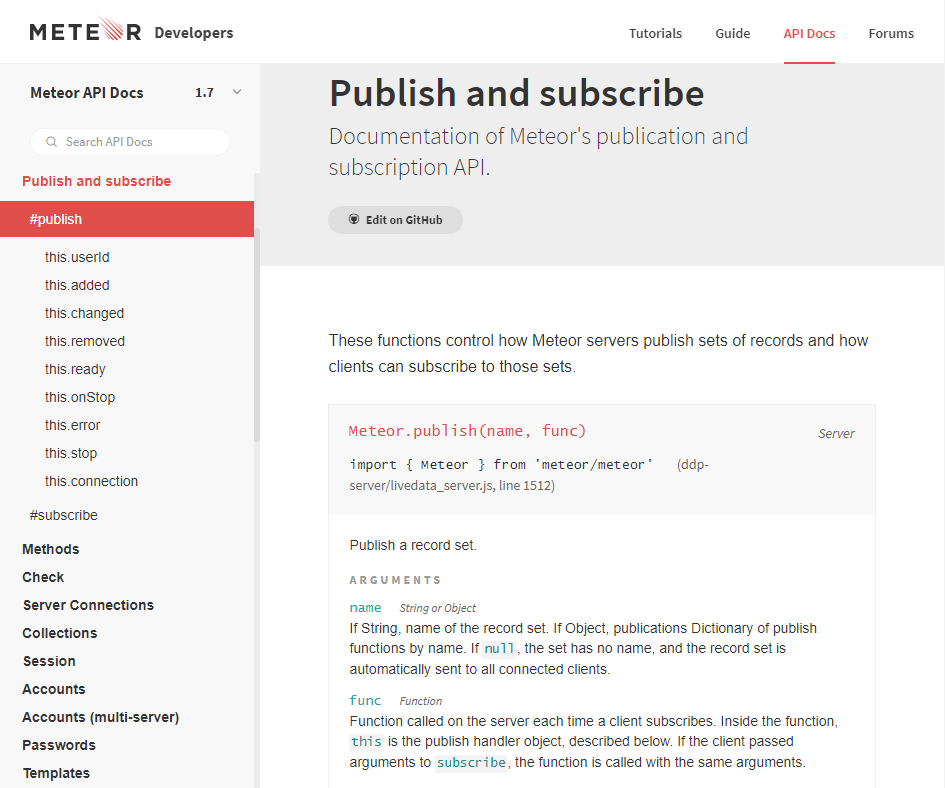
\includegraphics[width=\textwidth,height=\textheight,keepaspectratio]{doc_meteor.png} 
        \caption{Dokumentacja projektu Meteor \newline źródło: https://docs.meteor.com/\#/full/}
      \end{figure}

    \subsection{Próg wejścia}
      Meteor posiada wyższy próg wejścia niż pozostałe frameworki, ponieważ jest on całym ekosystemem wykorzystującym własne narzędzia.
      Posiada własny menadżer modułow Atmosphere, który w prawdzie posiada ogromną ilość komponentów wspierających wybrane funkcjonalności, ale nie są one tak popularne jak te z Npm.
      Jednak w przeciwieństwie do Npm aby umieścić moduł w Atmosphere musi on zostać zaakceptowany przez deweloperów odpowiedzialnych za biblioteke wprowadzając pewien stopień weryfikacji.
      Poprzez dostarczenie wielu gotowych rozwiązań Meteor posiada bardzo sztywny, specyficzny sposób wytwarzania projektu.
      Przy pierwszym kontakcie wiele konceptów jest niejasnych i odnaleźenie się w nich może sprawiać trudność. 
      Do wytwarzania najprostrzych projektów musimy posiadać wiedzę o wielu elementach środowika, które nie są wykorzystywana w żadnym innym rozwiązaniu.
      Ponieważ Meteor jest znacząco inny od pozostałych frameworków nie potrzebujemy mięć dużej wiedzy o technologii Node.js - wystarczy nam javaScript.

    \subsection{Warstwa widoku}
      Meteor po stronie widoku wspiera aplikacje napisane w React, Angular oraz silnik Blaze.
      Do działania na platformach mobilnych wykorzystuje silnik Cordova lub React Native.
      W repozytorium modułów atmosphere możemy znaleźć w pełni zaimplementowane koponenty służące do autoryzacji, wyświetlania filmów czy bibliotek zdjeć.
      Meteor kompiluje stworzone pliki html używając narzędzia Spacebars.
      Silnik Blaze zapewnia pełna synchronizacje (reaktywność) warstwy widoku oraz bazy danych (Minimongo).
      Obiekty reaktywne to obiekt sesji oraz kolekcje MongoDB.
      Do stworzenia analizowanego projektu wykrozystałem silnik Blaze.

    \subsection{Warstwa bazy danych}
      Framework Meteor aktualnie może działać tylko z bazami danych MongoDB.
      Po stronie serwera technologia używa sterownika MongoDB, a po stronie klienta używa biblioteki Minimongo.
      Minimongo jest to uproszczony klient bazy MongoDB, dzięki któremu nie musimy obawiać się o synchronizacje danych między warstwą frontendu oraz backendu.
      Framework automatycznie propaguje zmiany bazy danych w obydwu kierunkach poprzez wykorzystanie websocketów, oraz aktualizuje widok naszej aplikacji u klienta.
      Dzięki temu unikamy potrzeby tworzenia architektury komunikacji oraz uzykujemy aplikacje, która w każdym momencie może odzwierciedlać swój faktyczny, globalny stan.
    
    \subsection{Ilość kodu}
      Ilość wytworzonych lini kodu to około 250.
      Większość z nich dotyczy bezpośrednio widoku, nie logiki aplikacji do której obsługi zostały wykorzystane gotowe moduly z repozytorium Atmosphere.
      Najbardziej przydatnimi feature'ami oferowanymi przez biblioteke są:
      \begin{itemize}
        \item Publish/subscribe - pozwalające na reaktywne programowanie zdarzeń oraz reakcji na ich zajście.
        \item Blaze oraz Tracker - silnik pozwalający na zarządzanie reaktywne danymi zarówno po stronie widoku oraz bazy danych bez potrzeby tworzenia reaktywnej logiki.
        \item Automatyczna obsługa oraz synchronizacjia bazy danych nawet w przypadku wielu użytkowników bez potrzeby tworzenia dodatkowej logiki.
        \item Użycie globalnej zmiennej Meteor w każdym miejscu w kodzie, która posiad dostęp do wszystkich części aplikacji.
        \item Wbudowana obsługa wielu strategi autoryzacji użytkownika.
        \item Framework wymaga wytworzenia wyjątkowo niewielkiej ilości kodu pozwalając na tworzenie projektów w mgnieniu oka.
      \end{itemize}

    \subsection{Rozszerzalność}
      We frameworku Meteor wytwarzamy aplikacjie działające jednocześnie po stronie serwera oraz klienta.
      Programując możemy rozgraniczyć pewien kod poprzez trzymanie plików odpowiednio w folderach server oraz client.
      Pozostałe pliki będą dostępne po obu stronach, dzięki czemu możemy skorzystać z większej ilości reużywalnych komponentów, ale też musimy uważać aby nie udostępnić wrażliwych części aplikacji do klienta.
      Szkielet projektu przedstawia się następująco:
      \begin{itemize}
        \item lib - ustawienia, konfiguracje globalne
        \item public - udostępnione zasoby serwera jak zdjęcia, filmy, pliki stylów
        \item server - kod źródłowy obsługiwany po stronie wyłącznie serwera
        \item client - kod źródłowy obsługiwany po stronie wyłącznie klienta
        \item ui - widoki aplikacji
        \item startup - skrypty startowe
      \end{itemize}
      Metor swoją sztywną architekturą wymusza prowadzenie kodu podzielonego na jak najmniejsze, a przy odpowiednim utrzymaniu reużywalne części.
      Dzięki automatycznej synchronizacji oraz wykorzystaniu reaktywnych zmiennych możemy uniknąć problemów z synchronizacją danych w poszczególnych elementach aplikacji, nawet przy rozbudowanych projektach.
      Framewok wspomaga wytwarzanie rozszerzalnych produktów, jednak przy nieumiejętnym zarządzaniu nie gwarantuje tego.      

    \subsection{Testowanie}
      Metor nie dostarcza wraz z frameworkiem żadnego własnego rozwiązania testującego.
      Na stronie dokumentacji rekomendowaną biblioteką jest Mocha.
      Jest to framework służący do pisania każdego rodzaju przypadków testowych.
      Należy określić porządane efekty oraz sposób jak mają zostać uzyskane i zapakować je w test suits oraz test cases.
      Po użyciu narzędzia otrzymano wyniki testów:
      \begin{figure}[!hb]
        \centering
        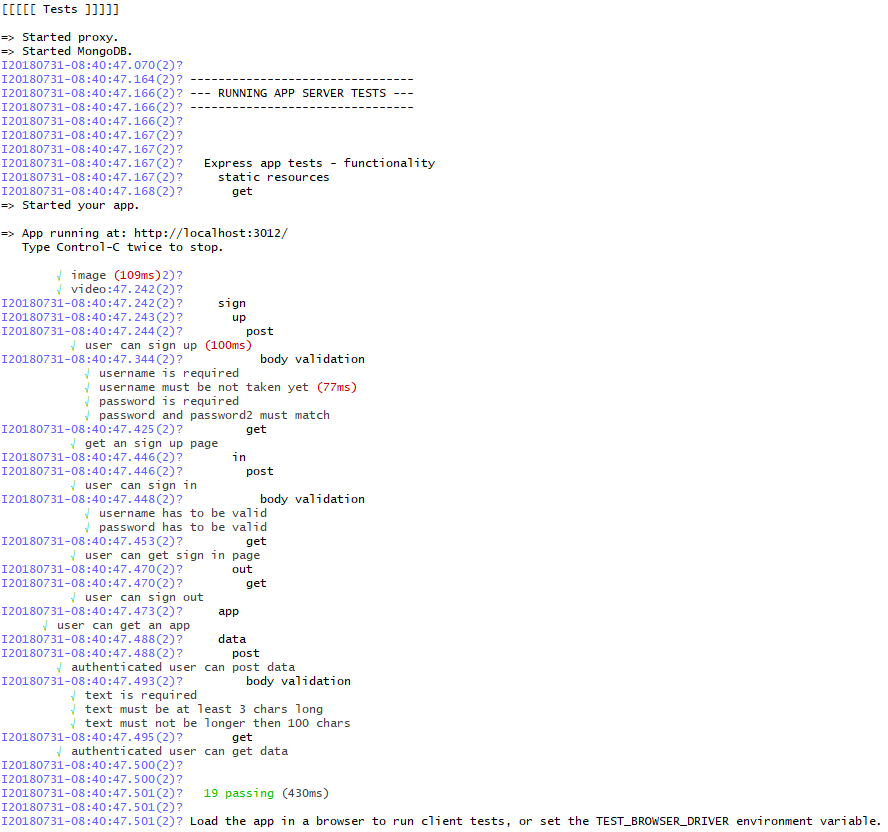
\includegraphics[width=\textwidth,height=\textheight,keepaspectratio]{test_meteor.png} 
        \caption{Testy frameworka Meteor przy użyciu biblioteki Mocha \newline źródło: opracowanie własne}
      \end{figure}

    \subsection{Testy sprawnościowe}
      Testy zostały przeprowadzone przy użyciu biblioteki Mocha.
      Podane wyniki reprezen-tują ilość przetworzonych zapytań w określonym czasie dla wybranych funkcjonalności.
      \smallskip
        \begin{center}
          \begin{tabular}{ | c | c | c | c | c | c | }
            \hline
            Okres czasu & Autoryzacja & Zapis danych tekstowych użytkownika & Zapytanie o zasób tekstowy użytkownika & Zapytanie o zasób obraz & Streaming multimediów video \\
            \hline
            2 sekundy & 172 & 193 & 187 & 178 & 37 \\
            \hline
            10 sekund & 859 & 957 & 935 & 1027 & 243 \\
            \hline
            30 sekund & 2437 & 2901 & 2655 & 2765 & 800 \\
            \hline
            Średnia ilość dla 1 sekundy & 83 & 96 & 90 & 95 & 26 \\
            \hline
          \end{tabular}
        \end{center}
      \bigskip\medskip

    \subsection{Testy obciążeniowe}
      Testy zostały przeprowadzone przy użyciu biblioteki Mocha.
      Podane wyniki reprezentują czas otrzymania odpowiedzi dla odpowiednich ilości zapytań w sekundach dla wybranych funkcjonalności.
      \smallskip
        \begin{center}
          \begin{tabular}{ | c | c | c | c | c | c | }
            \hline
            Ilości wysłanych równolegle zapytań & Autoryzacja & Zapis danych tekstowych użytkownika & Zapytanie o zasób tekstowy użytkownika & Zapytanie o zasób obraz & Streaming multimediów video \\
            \hline
            5 jednocześnie wysłanych zapytań & 0.885 & 0.098 & 0.071 & 0.064 & 0.249 \\
            \hline
            30 jednocześnie wysłanych zapytań & 4.372 & 0.621 & 0.412 & 0.299 & 1.42 \\
            \hline
            150 jednocześnie wysłanych zapytań & 19.006 & 3.598 & 2.073 & 0.739 & 4.923 \\
            \hline
            Średni czas dla 1 zapytania & 0.131 & 0.023 & 0.014 & 0.006 & 0.036 \\
            \hline
          \end{tabular}
        \end{center}
      \bigskip\medskip
    
\chapter{Podsumowanie}
  \section{Podsumowanie ocen}
    \subsection{Popularność}
      \smallskip
        \begin{center}
          \begin{tabular}{ | c | l | c | }
            \hline
            Framework & Opis & Ocena \\
            \hline
            Express & Express jest najbardziej rozpoznawanym frameworkiem środowiska Node.js. Nie ma żadnych problemów ze znalezieniem materiałów do nauki lub pomocy wśród społeczności. & 3 \\
            \hline
            Sails & Sails jest wciąż traktowany jako nowość aniżeli sprawdzone rozwiązanie (mimo komercyjnych zastosowań). Społeczność jest wciąż nie wielka. & 1\\
            \hline
            Meteor & Meteor posiada nie tak dużą jak Express lecz oddaną rzesze fanów. Możemy obserwować duża aktywność na forach poświęconych temu rozwiązaniu. Społeczność stale rozszerza framework, mimo że często jest traktowany jako ciekawostka. & 2 \\
            \hline
          \end{tabular}
        \end{center}
      \bigskip\medskip


      \begin{itemize}
        \item Express jest najbardziej rozpoznawanym frameworkiem środowiska Node.js. Nie ma żadnych problemów ze znalezieniem materiałów do nauki lub pomocy wśród społeczności.
        \item Sails jest wciąż traktowany jako nowość aniżeli sprawdzone rozwiązanie (mimo komercyjnych zastosowań). Społeczność jest wciąż nie wielka.
        \item Meteor posiada nie tak dużą jak Express lecz oddaną rzesze fanów. Możemy obserwować duża aktywność na forach poświęconych temu rozwiązaniu. Społeczność stale rozszerza framework, mimo że często jest traktowany jako ciekawostka. 
      \end{itemize}
      Oceny:
      \begin{itemize}
        \item Express - 3
        \item Sails - 1
        \item Meteor - 2
      \end{itemize}

    \subsection{Rozmiar}
      \begin{itemize}
        \item Express (18.1 mb) utrzymany w konwencji minimalnego frameworku, zawieraj-ącego tylko niezbędne moduły wypada najlepiej pod wzgłędem rozmiaru wytworzonej aplikacji.
        \item Sails (177 mb) znajduję się na drugim miejscu z nieco większym rozmiarem spowodowanym większą automatyzacją projektu.
        \item Meteor (454 mb) z powodu potrzeby posiadania środowiska frameworka znacznie odbiega od pozostałych rozwiązań pod kątem rozmiaru.
      \end{itemize}
      Oceny:
      \begin{itemize}
        \item Express - 3
        \item Sails - 2
        \item Meteor - 1
      \end{itemize}
      
    \subsection{Dokumentacja}
      \begin{itemize}
        \item Express w porównaniu do pozostałych rozwiązań posiada strone dokumentacji, która wydaje się być uboga, opisująca tylko podstawowe zagadnienia.
        \item Sails posiada bardzo czytelna i bogata dokumentacje. Łatwo znaleźć w niej informacje dla początkujących oraz zaawansowanych użytkowników.
        \item Meteor również posiada bardzo przyzwoita dokumentacje, zawierającą dokładne wytłumaczenia konceptów, a nawet filmy instruktarzowe.
      \end{itemize}
      Oceny:
      \begin{itemize}
        \item Express - 2
        \item Sails - 3
        \item Meteor - 3
      \end{itemize}
      
    \subsection{Próg wejścia}
      \begin{itemize}
        \item Express cechuje się zależnym progiem wejścia od skomplikowania projektu. Dla prostych przypadków jest on niski, a dla skomplikowanych znacząco rośnie.
        \item Sails nawet dla dużych, skomplikowanych projektów nie wymaga znacznie większej wiedzy poza podstawowymi konceptami. 
        \item Meteor posiada znacznie wyższy próg wejścia. Wprowadza bardzo wiele nowych ideii, zupełnie innych od tych znanych ze środowiska Node.js.
      \end{itemize}
      Oceny:
      \begin{itemize}
        \item Express - 2
        \item Sails - 3
        \item Meteor - 1
      \end{itemize}
      
    \subsection{Warstwa widoku}
      \begin{itemize}
        \item Express wspiera po stronie widoku aplikacje napisane w dowolnych technologiach frontendowych. Po stronie frameworku oferuję template rendering przy pomocy ogromnej ilości silników.
        \item Sails jako że został zbudowany na Express wspiera dokładnie te same rozwiąza-nia.
        \item Meteor posiada dedykowane, bardzo proste w obsłudzę rozwiązanie Blaze, które w pełni implementuje reaktywne zmiany widoku. Wspiera również aplikacje frameworków React oraz Angular.
      \end{itemize}
      Oceny:
      \begin{itemize}
        \item Express - 2
        \item Sails - 2
        \item Meteor - 3
      \end{itemize}
      
    \subsection{Warstwa bazy danych}
      \begin{itemize}
        \item Express po stronie frameworka nie oferuje żadnego wsparcia bazy danych. Należy użyć zewnętrznych rozwiązań.
        \item Sails używa biblioteki Waterline dostarczając bardzo prostego, zunifikowanego interfejsu do obsługi bazy danych.
        \item Meteor bardzo silnie został zintegrowany z bazą danych MongoDB, dzięki czemu zapewnia automatyczną synchronizację dla globalnego stanu aplikacji.
      \end{itemize}
      Oceny:
      \begin{itemize}
        \item Express - 1
        \item Sails - 3
        \item Meteor - 3
      \end{itemize}
      
    \subsection{Ilość kodu}
      \begin{itemize}
        \item Express (około 500) posiada najmniejszą ilość feature'ów oraz wymaga największej ilości kodu.
        \item Sails (około 400) cechuje się bardziej konfiguracją dostępnych rozwiązań niż tworzeniem logiki. 
        \item Meteor (około 250) znacznie odstaje od pozostałych rozwiązań. Możliwość użycia gotowych, skonfigurowanych modułów pozwala na stworznie aplikacji przy minimalnej ilości pracy.
      \end{itemize}
      Oceny:
      \begin{itemize}
        \item Express - 1
        \item Sails - 2
        \item Meteor - 3
      \end{itemize}
      
    \subsection{Rozszerzalność}
      \begin{itemize}
        \item Express pozwala na uzyskanie rozszerzalności zależnie tylko i wyłacznie od zastosowanych technik i umiejętności programistycznych użytkownika.
        \item Sails oferując sztywną architekture oraz możliwość łatwego wprowadzania zmian poprzez konfiguracje nie tworzenie logiki pozwala na łatwe uzyskanie skalowalnego projektu.
        \item Meteor wymusza prowadzenie kodu w określonej strukturze jednak nieumiejęte zarządzanie projektem może stworzyć problemy z rozszerzalnością.
      \end{itemize}
      Oceny:
      \begin{itemize}
        \item Express - 1
        \item Sails - 3
        \item Meteor - 2
      \end{itemize}

    \subsection{Testowanie}
      \begin{itemize}
        \item Express nie oferuje modułów przeznaczonych do testowania. Należy skorzystać z zewnętrznych rozwiązań.
        \item Sails nie wprowadza żadnych usprawnień w odniesieniu do Expressa odnośnie modułów testujących. Należy skorzystać z zewnętrznego rozwiązania.
        \item Meteor nie posiada zintegrowanych metod testujących kod. Dokumentacja wskazuję biblioteke mocha oraz prezętuje przypadki jej użycia.
      \end{itemize}
      Oceny:
      \begin{itemize}
        \item Express - 1
        \item Sails - 1
        \item Meteor - 1
      \end{itemize}
      
    \subsection{Testy sprawnościowe}
      \begin{itemize}
        \item Express (średnio 166 zapytań na sekunde) uzyskał znacznie lepsze wyniki od pozostałych frameworków w testach sprawnościowych. Ilość obsłużonyh zapytań była około 2 krotnie większa.
        \item Sails (średnio 95 zapytań na sekunde) osiągnął wyniki znacznie słabsze od Expressa, ale wciąż lepsze od Meteora.
        \item Meteor (średnio 78 zapytań na sekunde) uzyskał najmniej korzystne wyniki ze wszystkich testowanych rozwiązań.
      \end{itemize}
      Oceny:
      \begin{itemize}
        \item Express - 3
        \item Sails - 2
        \item Meteor - 1
      \end{itemize}
      
    \subsection{Testy obciążeniowe}
      \begin{itemize}
        \item Express (0.02 sek średni czas odpowiedzi na 1 zapytanie) wykazuję się również największą sprawnością jeśli chodzi o przetwarzanie wielu zapytań przychodzących równocześnie.
        \item Sails (0.04 sek średni czas odpowiedzi na 1 zapytanie) uzyskał średni czas odpowiedzi dwukrotnie dłuższy niż w przypadku Expressa.
        \item Meteor (0.04 sek średni czas odpowiedzi na 1 zapytanie) osiągnął takie same rezultaty jak Sails.
      \end{itemize}
      Oceny:
      \begin{itemize}
        \item Express - 3
        \item Sails - 2
        \item Meteor - 2
      \end{itemize}
      
    \subsection{Końcowe oceny}
      Po przeprowadzonej analizie frameworków, wyniki zostały zebrane w poniższej tabeli, a końcowe oceny wyliczone ze wzoru:
      Podstawiając pod wzór:
      \newline
      \[\text{\Large$O = \frac{\sum_{i=1}^{n} p_{i} * w_{i}}{sw}$}\]
      \newline
      \newline
      gdzie:
      \begin{description}
        \item[O] - ocena końcowa
        \item[n] - ilość parametrów
        \item[p] - ocena parametru
        \item[w] - waga parametru
        \item[sw] - suma wag parametrów
      \end{description}
      \iffalse
        Obliczenia:
        e = (3*3+1*3+3*2+1*2+2*2+2*1+2*1+3*1+2*1+3*3+3*3)/25 = 2.04
        s = (3*1+1*2+3*3+1*3+2*2+2*3+2*2+3*3+2*1+3*2+3*2)/25 = 2.16
        m = (3*2+1*1+3*3+1*1+2*3+2*3+2*3+3*2+2*1+3*1+3*2)/25 = 2.08
      \fi
      Uzyskane oceny:
      \smallskip
        \begin{center}
          \begin{tabular}{ | c | c | c | c | c | }
            \hline
            Parametr & Waga & Express & Sails & Meteor \\
            \hline
            Popularność & 3 & 3 & 1 & 2 \\
            \hline
            Rozmiar & 1 & 3 & 2 & 1 \\
            \hline
            Dokumentacja & 3 & 2 & 3 & 3 \\
            \hline
            Próg wejścia & 1 & 2 & 3 & 1 \\
            \hline
            Warstwa widoku & 2 & 2 & 2 & 3 \\
            \hline
            Warstwa bazy danych & 2 & 1 & 3 & 3 \\
            \hline
            Ilość kodu & 2 & 1 & 2 & 3 \\
            \hline
            Rozszerzalność & 3 & 1 & 3 & 2 \\
            \hline
            Testowanie & 2 & 1 & 1 & 1 \\
            \hline
            Testy sprawnościowe & 3 & 3 & 2 & 1 \\
            \hline
            Testy obciążeniowe & 3 & 3 & 2 & 2 \\
            \hline
            \setrow{\bfseries}Ocena Końcowa & - & 2.04 & 2.16 & 2.08 \\
            \hline
          \end{tabular}
        \end{center}
      \bigskip\medskip
      Ponieważ końcowe oceny niezanczenie się od siebie różnią warto wskazać zastosowania, w których dany framework bedzie najbardziej odpowiedni.

  \section{Wskazywane zastosowania}
    \subsection{Express}
      Express nadaje się idealnie to rozwiązań opracowywanych przez niewielkie zespoły deweloperskie, które nie rozrosną się do ogromnych projektów lub zostaną zaprojektowane jako wiele mikroserwisów z powodu braku ściśle określonych zasad architektury. 
      Brak wyraźnie określonych standardów wpływa na możliwe problemy z rozwojem projektu. 
      Oferuje bardzo szybkie przetwarzanie nawet przy dużym obciążeniu serwera, w związku z czym jest w stanie obsłużyć ogromną ilość jednoczesnych lub ciągle przychodzących połączeń.

    \subsection{Sails}
      Analiza wykazała że Sails uzyskał najlepszą ocene, otrzymując głównie pośrednie oceny poszczególnych parametrów - wydaje się być najbardziej uniwersalnym wyborem.
      Sprawdza się on dla wielu rozwiązań, ale jest naprawde ponadprzeciętny jeśli chodzi o projekty podatne na ciągłe zmiany i rozszerzenia, z powodu nacisku na konfigurowalność, a nie wytwarzanie kodu biznesowego.
      Doskonale sprawdza się przy aplikacjiach czasu rzeczywistego, streamingu oraz nawet serwerach gier wideo.

    \subsection{Meteor}
      Dostarczając wysoko zautomatyzowany proces deweloperski Meteor gwarantuje szybkie wytwarzanie prototypów czy MVP (ang. minimum viable product), które mogą być wysokoużyteczne w projektach startupowych, gdzie ponad niezawodne działanie ważne jest rozeznanie rynku i prezentacja produktu.
      Dodatkowe wsparcie platform mobilnych na podstawie tego samego kodu, chociaż nie zapewnia wysoce wydajnego działania pozwala sprawdzić zainteresowanie aplikacją bez potrzeby ponoszenia dodatkowych kosztów.
      Możemy oczywiście wytwarzać końcowe, docelowe produkty przy użyciu tej technologii, ale musimy być świadomi możliwego spadku jakości użytkowania oraz że zapewniona przez framework funkcjonalność (np. automatyczna synchronizacja baz danych) może okazać się wąskim gardłem kiedy aplikacja rozrośnie się do dużo większej skali.

\addcontentsline{toc}{chapter}{Bibliografia}

\begin{thebibliography}{99}
  \bibitem{Brown}
    E. Brown \newline
    \textit{"Web Development with Node and Express", 2014}

  \bibitem{Mardan}
    Azat Mardan \newline
    \textit{"Express.js Guide: The Comprehensive Book on Express.js", 2016}

  \bibitem{StrongLoop}
    StrongLoop \newline
    \textit{dokumentacja Express, 2017 \newline źródło: https://expressjs.com/en/4x/api.html}

  \bibitem{McNeil&Nathan}
    Mike McNeil, Irl Natha \newline
    \textit{"Sails.js in Action", 2017}

  \bibitem{Shahid}
    Shahid Shaikh \newline
    \textit{"Sails.js Essentials", 2016}

  \bibitem{McNeil}
    Mike McNeil \newline
    \textit{dokumentacja Sails, 2017 \newline źródło: https://sailsjs.com/documentation/reference}

  \bibitem{Strack}
    Isaac Strack \newline
    \textit{"Getting Started with Meteor JavaScript Framework", 2012}

  \bibitem{Vogelsteller&Strack&Reyna}
    Fabian Vogelsteller, Isaac Strack, Marcelo Reyna \newline
    \textit{"Meteor: Full-Stack Web Application Development", 2016}

  \bibitem{MDG}
    Meteor Development Group \newline
    \textit{dokumentacja Meteor API, 2017 \newline źródło: https://docs.meteor.com/\#/full/}

  \bibitem{Onodi}
    Node.js Foundation \newline
    \textit{dokumentacja języka programowania Node.js, 2017 \newline źródło: https://nodejs.org/en/docs/}

  \bibitem{Wolff}
    Eberhard Wolff \newline
    \textit{"Microservices: Flexible Software Architecture", 2016}

  \bibitem{Zeidman}
    Bob Zeidman \newline
    \textit{"The Software IP Detective's Handbook: Measurement, Comparison, and Infringement Detection", 2011}
    
  \bibitem{Rauch}
    Guillermo Rauch \newline
    \textit{"7 Principles of Rich Web Applications", 2014}

\end{thebibliography}

\addcontentsline{toc}{chapter}{Spis rysunków}

\listoffigures

\end{document}